\documentclass[review]{elsarticle}
%DIF LATEXDIFF DIFFERENCE FILE
%DIF DEL main.tex                                                       Fri Mar  5 23:51:09 2021
%DIF ADD C:\Users\mehme\Documents\GitHub\2020-turkmen-ml-msr\main.tex   Thu Feb 25 18:32:55 2021

\usepackage{multirow}
\usepackage{lineno}
\usepackage{xspace}
%\usepackage{subfig}
\modulolinenumbers[5]

%% Journal name here
\journal{Annals of Nuclear Energy}

%% `Elsevier LaTeX' style
\bibliographystyle{elsarticle-num}
%%%%%%%%%%%%%%%%%%%%%%%

%%%% packages and definitions (optional)
\usepackage{placeins}
\usepackage{booktabs} % nice rules (thick lines) for tables
\usepackage{microtype} % improves typography for PDF
\usepackage{hhline}
\usepackage{amsmath}
\usepackage{graphicx}
\usepackage{subcaption}
\usepackage{pdflscape}

%DIF 26a26
\usepackage{acronym} %DIF >
%DIF -------
\usepackage{booktabs}
\usepackage{threeparttable, tablefootnote}

\usepackage{tabularx}
\usepackage[table]{xcolor}
%DIF 31-35d32
%DIF <
%DIF < %% Special typesetting for Cyclus
%DIF < \newcommand{\Cyclus}{\textsc{Cyclus}\xspace}%
%DIF < \newcommand{\Cycamore}{\textsc{Cycamore}\xspace}%
%DIF < \graphicspath{{images/}}
%DIF -------

% tikz %
\usepackage{tikz}
\usetikzlibrary{positioning, arrows, decorations, shapes}

\usetikzlibrary{shapes.geometric,arrows}
\tikzstyle{process} = [rectangle, rounded corners, minimum width=3cm, minimum
height=1cm,text centered, draw=black, fill=blue!30]
\tikzstyle{object} = [ellipse, rounded corners, minimum width=3cm, minimum
height=1cm,text centered, draw=black, fill=green!30]
\tikzstyle{arrow} = [thick,->,>=stealth]

% hyperref %
\usepackage[hidelinks]{hyperref}
% after hyperref %
\usepackage{cleveref}
\usepackage{datatool}
\usepackage[acronym,toc]{glossaries}
%\newacronym{<++>}{<++>}{<++>}
\newacronym{AB}{AB}{AdaBoost}
\newacronym{AI}{AI}{Artificial Intelligence}
\newacronym{ANN}{ANN}{Artificial Neural Network}
\newacronym{AP}{AP}{average precision}
\newacronym{B}{B}{Bagging}
\newacronym{BNB}{BNB}{BernoulliNB}
\newacronym{DT}{DT}{DecisionTree}
\newacronym{EALF}{EALF}{energy corresponding to average lethargy of neutrons causing fission}
\newacronym{EN}{EN}{ElasticNet}
\newacronym{ET}{ET}{ExtraTrees}
\newacronym{EVR}{EVR}{explained variance regression score}
\newacronym{GA}{GA}{Genetic Algorithm}
\newacronym{GB}{GB}{GradientBoosting}
\newacronym{GNB}{GNB}{GaussianNB}
\newacronym{HALEU}{HALEU}{High Assay Low Enriched Uranium}
\newacronym{HL}{HL}{average Hamming loss}
\newacronym{KN}{KN}{KNeighbors}
\newacronym{L}{L}{Lasso}
\newacronym{LL}{LL}{LassoLars}
\newacronym{Log}{Log}{Logistic}
\newacronym{LP}{LP}{LabelPropagation}
\newacronym{LRAPS}{LRAPS}{ranking-based average precision}
\newacronym{LRL}{LRL}{label ranking loss}
\newacronym{MAE}{MAE}{mean absolute error}
\newacronym{ML}{ML}{Machine Learning}
\newacronym{MLP}{MLP}{MultiLayerPerceptron}
\newacronym{MOGA}{MOGA}{Multi-Objective Genetic Algorithm}
\newacronym{MSE}{MSE}{mean square error}
\newacronym{MSR}{MSR}{Molten Salt Reactor}
\newacronym{MSRE}{MSRE}{Molten Salt Reactor Experiment}
\newacronym{NN}{NN}Neural Network}
\newacronym{NSGAIII}{NSGAIII}{non-dominated sorting genetic algorithm}
\newacronym{ORNL}{ORNL}{Oak Ridge National Laboratory}
\newacronym{P}{P}{Perceptron}
\newacronym{PM}{PM}{polynomial mutation}
\newacronym{R}{R}{Ridge}
\newacronym{RF}{RF}{RandomForest}
\newacronym{ROC_AUC}{MAE}{compute area under the receiver operating characteristic curve}
\newacronym{SBX}{SBX}{simulated binary crossover}
\newacronym{SGD}{SGD}{StochasticGradientDescent}
\newacronym{SV}{SV}{SupportVector}
\newacronym{SVM}{SVM}{support vector machine}
\newacronym{UNF}{UNF}{Used Nuclear Fuel}

\graphicspath{{../}}

\makeglossaries
%DIF PREAMBLE EXTENSION ADDED BY LATEXDIFF
%DIF UNDERLINE PREAMBLE %DIF PREAMBLE
\RequirePackage[normalem]{ulem} %DIF PREAMBLE
\RequirePackage{color}\definecolor{RED}{rgb}{1,0,0}\definecolor{BLUE}{rgb}{0,0,1} %DIF PREAMBLE
\providecommand{\DIFaddtex}[1]{{\protect\color{blue}\uwave{#1}}} %DIF PREAMBLE
\providecommand{\DIFdeltex}[1]{{\protect\color{red}\sout{#1}}}                      %DIF PREAMBLE
%DIF SAFE PREAMBLE %DIF PREAMBLE
\providecommand{\DIFaddbegin}{} %DIF PREAMBLE
\providecommand{\DIFaddend}{} %DIF PREAMBLE
\providecommand{\DIFdelbegin}{} %DIF PREAMBLE
\providecommand{\DIFdelend}{} %DIF PREAMBLE
\providecommand{\DIFmodbegin}{} %DIF PREAMBLE
\providecommand{\DIFmodend}{} %DIF PREAMBLE
%DIF FLOATSAFE PREAMBLE %DIF PREAMBLE
\providecommand{\DIFaddFL}[1]{\DIFadd{#1}} %DIF PREAMBLE
\providecommand{\DIFdelFL}[1]{\DIFdel{#1}} %DIF PREAMBLE
\providecommand{\DIFaddbeginFL}{} %DIF PREAMBLE
\providecommand{\DIFaddendFL}{} %DIF PREAMBLE
\providecommand{\DIFdelbeginFL}{} %DIF PREAMBLE
\providecommand{\DIFdelendFL}{} %DIF PREAMBLE
%DIF HYPERREF PREAMBLE %DIF PREAMBLE
\providecommand{\DIFadd}[1]{\texorpdfstring{\DIFaddtex{#1}}{#1}} %DIF PREAMBLE
\providecommand{\DIFdel}[1]{\texorpdfstring{\DIFdeltex{#1}}{}} %DIF PREAMBLE
\newcommand{\DIFscaledelfig}{0.5}
%DIF HIGHLIGHTGRAPHICS PREAMBLE %DIF PREAMBLE
\RequirePackage{settobox} %DIF PREAMBLE
\RequirePackage{letltxmacro} %DIF PREAMBLE
\newsavebox{\DIFdelgraphicsbox} %DIF PREAMBLE
\newlength{\DIFdelgraphicswidth} %DIF PREAMBLE
\newlength{\DIFdelgraphicsheight} %DIF PREAMBLE
% store original definition of \includegraphics %DIF PREAMBLE
\LetLtxMacro{\DIFOincludegraphics}{\includegraphics} %DIF PREAMBLE
\newcommand{\DIFaddincludegraphics}[2][]{{\color{blue}\fbox{\DIFOincludegraphics[#1]{#2}}}} %DIF PREAMBLE
\newcommand{\DIFdelincludegraphics}[2][]{% %DIF PREAMBLE
\sbox{\DIFdelgraphicsbox}{\DIFOincludegraphics[#1]{#2}}% %DIF PREAMBLE
\settoboxwidth{\DIFdelgraphicswidth}{\DIFdelgraphicsbox} %DIF PREAMBLE
\settoboxtotalheight{\DIFdelgraphicsheight}{\DIFdelgraphicsbox} %DIF PREAMBLE
\scalebox{\DIFscaledelfig}{% %DIF PREAMBLE
\parbox[b]{\DIFdelgraphicswidth}{\usebox{\DIFdelgraphicsbox}\\[-\baselineskip] \rule{\DIFdelgraphicswidth}{0em}}\llap{\resizebox{\DIFdelgraphicswidth}{\DIFdelgraphicsheight}{% %DIF PREAMBLE
\setlength{\unitlength}{\DIFdelgraphicswidth}% %DIF PREAMBLE
\begin{picture}(1,1)% %DIF PREAMBLE
\thicklines\linethickness{2pt} %DIF PREAMBLE
{\color[rgb]{1,0,0}\put(0,0){\framebox(1,1){}}}% %DIF PREAMBLE
{\color[rgb]{1,0,0}\put(0,0){\line( 1,1){1}}}% %DIF PREAMBLE
{\color[rgb]{1,0,0}\put(0,1){\line(1,-1){1}}}% %DIF PREAMBLE
\end{picture}% %DIF PREAMBLE
}\hspace*{3pt}}} %DIF PREAMBLE
} %DIF PREAMBLE
\LetLtxMacro{\DIFOaddbegin}{\DIFaddbegin} %DIF PREAMBLE
\LetLtxMacro{\DIFOaddend}{\DIFaddend} %DIF PREAMBLE
\LetLtxMacro{\DIFOdelbegin}{\DIFdelbegin} %DIF PREAMBLE
\LetLtxMacro{\DIFOdelend}{\DIFdelend} %DIF PREAMBLE
\DeclareRobustCommand{\DIFaddbegin}{\DIFOaddbegin \let\includegraphics\DIFaddincludegraphics} %DIF PREAMBLE
\DeclareRobustCommand{\DIFaddend}{\DIFOaddend \let\includegraphics\DIFOincludegraphics} %DIF PREAMBLE
\DeclareRobustCommand{\DIFdelbegin}{\DIFOdelbegin \let\includegraphics\DIFdelincludegraphics} %DIF PREAMBLE
\DeclareRobustCommand{\DIFdelend}{\DIFOaddend \let\includegraphics\DIFOincludegraphics} %DIF PREAMBLE
\LetLtxMacro{\DIFOaddbeginFL}{\DIFaddbeginFL} %DIF PREAMBLE
\LetLtxMacro{\DIFOaddendFL}{\DIFaddendFL} %DIF PREAMBLE
\LetLtxMacro{\DIFOdelbeginFL}{\DIFdelbeginFL} %DIF PREAMBLE
\LetLtxMacro{\DIFOdelendFL}{\DIFdelendFL} %DIF PREAMBLE
\DeclareRobustCommand{\DIFaddbeginFL}{\DIFOaddbeginFL \let\includegraphics\DIFaddincludegraphics} %DIF PREAMBLE
\DeclareRobustCommand{\DIFaddendFL}{\DIFOaddendFL \let\includegraphics\DIFOincludegraphics} %DIF PREAMBLE
\DeclareRobustCommand{\DIFdelbeginFL}{\DIFOdelbeginFL \let\includegraphics\DIFdelincludegraphics} %DIF PREAMBLE
\DeclareRobustCommand{\DIFdelendFL}{\DIFOaddendFL \let\includegraphics\DIFOincludegraphics} %DIF PREAMBLE
%DIF LISTINGS PREAMBLE %DIF PREAMBLE
\RequirePackage{listings} %DIF PREAMBLE
\RequirePackage{color} %DIF PREAMBLE
\lstdefinelanguage{DIFcode}{ %DIF PREAMBLE
%DIF DIFCODE_UNDERLINE %DIF PREAMBLE
  moredelim=[il][\color{red}\sout]{\%DIF\ <\ }, %DIF PREAMBLE
  moredelim=[il][\color{blue}\uwave]{\%DIF\ >\ } %DIF PREAMBLE
} %DIF PREAMBLE
\lstdefinestyle{DIFverbatimstyle}{ %DIF PREAMBLE
	language=DIFcode, %DIF PREAMBLE
	basicstyle=\ttfamily, %DIF PREAMBLE
	columns=fullflexible, %DIF PREAMBLE
	keepspaces=true %DIF PREAMBLE
} %DIF PREAMBLE
\lstnewenvironment{DIFverbatim}{\lstset{style=DIFverbatimstyle}}{} %DIF PREAMBLE
\lstnewenvironment{DIFverbatim*}{\lstset{style=DIFverbatimstyle,showspaces=true}}{} %DIF PREAMBLE
%DIF END PREAMBLE EXTENSION ADDED BY LATEXDIFF

\begin{document}
	%\input{highlights/highlights}
	\begin{frontmatter}
		\title{Machine Learning Application to
			Single Channel Design of Molten Salt Reactor}

		% Authors
		\author[uiuc]{Mehmet Turkmen\corref{corrauthor}}
\cortext[corrauthor]{Corresponding Author}
\ead{mturkmen@illinois.edu}
\author[uiuc]{Gwendolyn Chee}
\author[uiuc]{Kathryn D. Huff}




		% Institutes of the authors
		\address[uiuc]{Dept. of Nuclear, Plasma, and Radiological Engineering,
University of Illinois at Urbana-Champaign, Urbana, IL 61801}


		\begin{keyword}
			channel design \sep
			molten salt reactor \sep
			machine learning \sep
			optimization \sep
			simulation \sep
			Monte Carlo
		\end{keyword}

		\begin{abstract}

This study proposes an efficient, accelerated\DIFaddbegin \DIFadd{, }\DIFaddend and robust approach to design a nuclear reactor core from scratch, using state-of-the-art machine learning \gls{ML} techniques. We implemented the \DIFdelbegin \DIFdel{recommended }\DIFdelend approach into a \DIFdelbegin \DIFdel{single fuel
channel of a molten salt reactor (MSR) }\DIFdelend \DIFaddbegin \DIFadd{hypothetical channel of molten salt reactors }\DIFaddend to demonstrate the applicability of the method. We prepared a Python tool, named Plankton, which couples to a reactor physics code and \DIFdelbegin \DIFdel{the Multi-Objective Genetic Algorithm}\DIFdelend \DIFaddbegin \DIFadd{an optimization tool}\DIFaddend , and imports \gls{ML} methods. \DIFdelbegin \DIFdel{It }\DIFdelend \DIFaddbegin \DIFadd{The tool }\DIFaddend performs three consecutive phases: \DIFdelbegin \DIFdel{(i) }\DIFdelend reactor database generation, \DIFdelbegin \DIFdel{(ii) }\DIFdelend machine learning application, \DIFdelbegin \DIFdel{(iii) }\DIFdelend \DIFaddbegin \DIFadd{and }\DIFaddend design optimization. \DIFdelbegin \DIFdel{With the extra-trees method }\DIFdelend \DIFaddbegin \DIFadd{We identified the extra trees method as the best performing estimator among various }\gls{ML} \DIFadd{estimators. With the estimator}\DIFaddend , we found nine optimum designs \DIFaddbegin \DIFadd{in total, one }\DIFaddend for each fuel-salt pair\DIFaddbegin \DIFadd{, }\DIFaddend and estimated all the performance metrics of the \DIFdelbegin \DIFdel{optimum designs within a prediction
error of }\DIFdelend \DIFaddbegin \DIFadd{designs with a }\DIFaddend $<$5\% \DIFdelbegin \DIFdel{with respect }\DIFdelend \DIFaddbegin \DIFadd{prediction error compared }\DIFaddend to their actual values. \DIFdelbegin \DIFdel{U-Pu fuel mixed with NaCl
salt as well as LiF-BeF$_2$ salt gave the promising results , yielding }\DIFdelend \DIFaddbegin \DIFadd{U-Pu-NaCl fuel-salt gave promising results with }\DIFaddend the highest conversion ratio, the most negative feedback coefficient, and the lowest fast flux.

\end{abstract}

	\end{frontmatter}
	\glsresetall

	%% Shows line numbers
	\linenumbers

	\section{Introduction}

    Current applications of learning-based techniques in nuclear engineering indicate that \gls{AI} will soon undertake the role of reactor designers in optimizing the designs of current and future reactors. \gls{AI} methods, more specifically \gls{ML}, have already become important to most sub-fields of nuclear science and engineering (e.g., in-core fuel management, reactor safety, flow regime prediction, and radiation protection) to achieve an optimal core loading map, to make nuclear reactors safer, to quickly comprehend flow data, and to accurately identify critical isotopes in nuclear materials. In this context, recently published two review papers \cite{Gomez2020, Nissan2019} showed the potential, competence, and importance of these methods by exploring the recent studies on the use of learning-based methods in nuclear science and relevant fields. The articles also probed the suitability of \DIFaddbegin \DIFadd{the }\DIFaddend commonly used algorithms and algorithm selection criteria. However, \gls{AI}/\gls{ML} has not contemplated as an option to seek \DIFdelbegin \DIFdel{optimal design features }\DIFdelend \DIFaddbegin \DIFadd{to find optimal designs }\DIFaddend of nuclear reactor cores despite being a proven technique for optimization. Instead, \DIFdelbegin \DIFdel{the methods
widely employed for reactor core design optimization are }\DIFdelend iterative approaches such as individual parameter searches and \DIFdelbegin %DIFDELCMD < \gls{GA}%%%
\DIFdelend \DIFaddbegin \DIFadd{evolutionary algorithms have been widely employed for reactor core design optimization}\DIFaddend .

    Among \DIFdelbegin \DIFdel{the }\DIFdelend parametric studies recently reported, Wei \emph{et al.} \cite{Wei2018} investigated several critical feature parameters of a \gls{MSR} channel by parameter interpolation using KENO-VI in SCALE 6.1 \cite{scale2020}. In the study, \DIFdelbegin \DIFdel{the }\DIFdelend critical feature parameters are the fuel \DIFdelbegin \DIFdel{material}\DIFdelend \DIFaddbegin \DIFadd{type}\DIFaddend , $^{6}$Li concentration, composition of fuel \DIFdelbegin \DIFdel{material}\DIFdelend \DIFaddbegin \DIFadd{type}\DIFaddend , channel geometry, moderator \DIFdelbegin \DIFdel{,
moderator density}\DIFdelend \DIFaddbegin \DIFadd{and its density, }\DIFaddend and salt operation temperature. The research showed that $^{6}$Li has a strong effect on \DIFdelbegin \DIFdel{the }\DIFdelend criticality. In all different shapes of fuel channels, Wei \emph{et al.} \cite{Wei2018} observed that the turning point from under-moderation to over-moderation for the multiplication factor ($k$) is at a pitch to channel ratio ($P/D$) between 2 and 4, and a fuel volume fraction between 0 and 0.1. Increasing the amount of moderator resulted in an increase in $k$, but then further increase caused a decrease. Meanwhile, the temperature coefficient changes from negative to positive for pitch $>$ 12 cm.

    Anderson \emph{et al.} \cite{Anderson2019} assessed the importance of several parameters (fissile enrichment, lattice pitch, salt-moderator ratio\DIFdelbegin \DIFdel{and }\DIFdelend \DIFaddbegin \DIFadd{, and the }\DIFaddend number of fuel channels) in \DIFdelbegin \DIFdel{the }\DIFdelend \DIFaddbegin \DIFadd{a }\DIFaddend \gls{MSR} core by looking into the change of \DIFdelbegin \DIFdel{the
}\DIFdelend fission and removal transition matrices. In that work, the results showed that some of these parameters have an increasing impact on the average relative difference of transition matrices while \DIFdelbegin \DIFdel{the some }\DIFdelend \DIFaddbegin \DIFadd{others }\DIFaddend have a decreasing effect.

    The common deficiency of both studies is the neglect of strong interdependence of \DIFdelbegin \DIFdel{the }\DIFdelend \DIFaddbegin \DIFadd{those }\DIFaddend investigated parameters, by carrying out only \DIFaddbegin \DIFadd{a }\DIFaddend single parametric study. The effect of a single parameter on performance metrics (multiplication factor, conversion ratio, reactivity feedback coefficient, etc.) can be either beneficial or detrimental. As for more than one parameter, correlations between parameters can be seen as \DIFdelbegin \DIFdel{super positioning}\DIFdelend \DIFaddbegin \DIFadd{superpositioning}\DIFaddend , canceling out another, or acting on each other up to some extent. Correspondingly, such multi-parameter optimizations would require more sophisticated searching techniques like \DIFdelbegin %DIFDELCMD < \gls{GA}%%%
\DIFdel{, Particle Swarm, and }%DIFDELCMD < \gls{ANN} %%%
\DIFdelend \DIFaddbegin \DIFadd{genetic algorithm, particle swarm, and simulated annealing }\DIFaddend methods. Unlike parametric \DIFdelbegin \DIFdel{study}\DIFdelend \DIFaddbegin \DIFadd{studies}\DIFaddend , these sophisticated optimization techniques are very useful in finding optimal parameters, particularly for multi-objective problems\DIFaddbegin \DIFadd{, }\DIFaddend and are a common and effective way of determining optimal core loading maps \cite{Nissan2019}.

    In \DIFaddbegin \DIFadd{the }\DIFaddend case of using evolutionary algorithms in core designs, Kumar and Tsvetkov \cite{Kumar2015} used a \DIFdelbegin \DIFdel{Genetic Algorithm }\DIFdelend \DIFaddbegin \gls{GA} \DIFaddend method coupled to \DIFdelbegin \DIFdel{Regression Splines
}\DIFdelend \DIFaddbegin \DIFadd{regression splines }\DIFaddend to optimize several performance metrics such as multiplication factor, fast fission factor, thermal efficiency, and \DIFdelbegin \DIFdel{burnup }\DIFdelend \DIFaddbegin \DIFadd{burn up }\DIFaddend in the design of \DIFdelbegin \DIFdel{the }\DIFdelend Gas Cooled Fast Breeder reactor. \DIFdelbegin \DIFdel{This }\DIFdelend \DIFaddbegin \DIFadd{That }\DIFaddend method interpolates intermediate values of \DIFdelbegin \DIFdel{the
}\DIFdelend parameters and metrics. \DIFdelbegin \DIFdel{For }\DIFdelend \DIFaddbegin \DIFadd{Regarding }\DIFaddend a fuel pin cell, \DIFdelbegin \DIFdel{the optimal values of the }\DIFdelend \DIFaddbegin \DIFadd{optimal design values of }\DIFaddend radius, enrichment fraction, mass flow rate, and coolant temperature at the inlet were found to be 0.22 cm, 18.5 wt. \%, 63.5  $^o$C, and 35.9 kg/s, respectively. Zeng \emph{et al.} \cite{Zeng2020} performed a multi-objective optimization to the Advanced Burner Test Reactor (ABTR) core, a sodium-cooled fast test reactor (SFR), to get \DIFdelbegin \DIFdel{a final }\DIFdelend \DIFaddbegin \DIFadd{an ultimate }\DIFaddend core design. In \DIFdelbegin \DIFdel{the }\DIFdelend \DIFaddbegin \DIFadd{that }\DIFaddend work, an integrated version of the US Department of Energy's Nuclear Energy Advanced Modeling and Simulation (NEAMS) Workbench \cite{neams2019} along with \gls{GA} was used for core modeling and optimization. Although they found about 3150 optimal core designs within Pareto front solutions by optimizing \DIFdelbegin \DIFdel{the }\DIFdelend reactivity swing, Pu mass feed, core volume, core power, and peak fast flux, only six candidate designs passed their performance criteria based on \DIFdelbegin \DIFdel{the }\DIFdelend \DIFaddbegin \DIFadd{their }\DIFaddend defined constraints.

    \DIFaddbegin \DIFadd{Two other important studies \mbox{%DIFAUXCMD
\cite{pereira1999, pereira2003} }\hspace{0pt}%DIFAUXCMD
investigated a hypothetical reactor design in a cylindrical fuel rod geometry (i.e., composed of a moderator, clad, and fuel regions) to validate the }\gls{GA} \DIFadd{applicability and to make a comparison with classical linear optimization methods. In the first study, only two continuous feature parameters were considered for optimization. Optimal designs were completed using 3500 reactor simulations (100 populations and 35 generations). Later, a more complex version of the previous problem was repeated with continuous and discrete variables, very identical to our problem from the aspects of types and number of feature parameters. Optimization results were obtained with 150000 reactor simulations (300 populations and 500 generations).
}

    \DIFaddend Recently published studies \cite{Kim2018, Kim2020} reported the results of \DIFdelbegin \DIFdel{the
}\DIFdelend \DIFaddbegin \DIFadd{an }\DIFaddend assembly and core design at the Kyoto University Critical Assembly \DIFdelbegin \DIFdel{by means of
}\DIFdelend \DIFaddbegin \DIFadd{through }\DIFaddend an \gls{ANN} coupled to MCNP6 \cite{mcnp2017}. These studies are similar to fuel loading pattern optimization studies in terms of \DIFaddbegin \DIFadd{the }\DIFaddend optimization approach. In these works, \DIFdelbegin \DIFdel{various }\DIFdelend \DIFaddbegin \DIFadd{different }\DIFaddend core materials, \DIFdelbegin \DIFdel{numbers }\DIFdelend \DIFaddbegin \DIFadd{the number }\DIFaddend of fuel regions, and fuel assembly types were defined as vital feature parameters whereas fast flux and multiplication factor were the target metrics to be optimized.

    Regarding the use of \gls{ML} methods in depletion prediction of reactor applications, Bae \emph{et al.} \cite{Bae2020} successfully predicted Pressurized Water Reactor (PWR) \gls{UNF} composition by training the dense neural network in the Keras \cite{keras2015}. They showed that their proposed model outperforms the average recipe method, one of the transmutation methods which supplies neutronic calculations externally to the nuclear fuel cycle simulators, by yielding less than 1\% error for the \gls{UNF} inventory decay heat and activity and less than 5\% error for the important isotopes.

    As discussed previously, parametric studies which handle all feature variables independently ignore \DIFaddbegin \DIFadd{the }\DIFaddend complex interdependence of these variables and evaluate performance metrics \DIFdelbegin \DIFdel{of a design }\DIFdelend by changing only one \DIFdelbegin \DIFdel{of the feature variables }\DIFdelend \DIFaddbegin \DIFadd{feature variable }\DIFaddend at a time, thus fixing others\DIFdelbegin \DIFdel{whereas }\DIFdelend \DIFaddbegin \DIFadd{. Meanwhile, }\DIFaddend evolutionary algorithms suffer from the choices of optimizer \DIFdelbegin \DIFdel{hyper-parameters }\DIFdelend \DIFaddbegin \DIFadd{hyperparameters }\DIFaddend such as population size, number of generations\DIFaddbegin \DIFadd{, }\DIFaddend and cross-over rate \DIFdelbegin \DIFdel{, }\DIFdelend since it is unlikely to determine exactly what these parameters would be without making a preliminary calculation. \DIFaddbegin \DIFadd{Additionally, these optimization techniques do not provide any flexibility to the designers, such as making optimization without running reactor simulator again when constraints are changed. }\DIFaddend This hence results in excessive usage of computational resources. Furthermore, optimization methods \DIFdelbegin \DIFdel{frequently }\DIFdelend \DIFaddbegin \DIFadd{occasionally }\DIFaddend converge to local instead of global optima fail to achieve ideal designs that are eliminated by the optimizer's elimination and/or selection criteria. At this point, \DIFaddbegin \DIFadd{if sufficient data is supplied, }\DIFaddend the use of learning-based methods seems rational \DIFdelbegin \DIFdel{for the design of a }\DIFdelend \DIFaddbegin \DIFadd{to design a nuclear }\DIFaddend reactor because of their exceptional ability to \DIFdelbegin \DIFdel{fully scan every inch of the parameter space without missing the global optimum}\DIFdelend \DIFaddbegin \DIFadd{accurately predict performance metrics and appropriate to use with optimization tools as a reactor simulator}\DIFaddend .

    The \gls{ML} methods, which have not been considered for the sole design of a reactor core so far, will be the best option in this regard. \DIFdelbegin \DIFdel{Accordingly, we
recommend using }\DIFdelend \DIFaddbegin \DIFadd{This article compares various }\DIFaddend \gls{ML} methods \DIFdelbegin \DIFdel{to estimate the optimal values of reactor
design parameters by predicting performance metrics without running neutron transport calculations}\DIFdelend \DIFaddbegin \DIFadd{in terms of performance scores and recommends employing these methods in place of neutron transport codes for the prediction of performance metrics}\DIFaddend . This research \DIFdelbegin \DIFdel{demonstrate }\DIFdelend \DIFaddbegin \DIFadd{demonstrates }\DIFaddend that the proposed method predicts performance metrics more accurately and quickly than \DIFdelbegin \DIFdel{current
}\DIFdelend \DIFaddbegin \DIFadd{the existing }\DIFaddend optimization techniques.

	\section{Methodology}

    In this section, we described how to apply \DIFdelbegin \DIFdel{the }\DIFdelend \gls{ML} methods to design a reactor core. We followed a \DIFaddbegin \DIFadd{strict }\DIFaddend methodology consisting of three separate phases: (1) database generation, (2) machine learning, and (3) design optimization. For this, we developed a Python tool, called Plankton. The Plankton produces training and \DIFdelbegin \DIFdel{testing }\DIFdelend \DIFaddbegin \DIFadd{test }\DIFaddend datasets for given feature parameters, \DIFdelbegin \DIFdel{determines a }%DIFDELCMD < \gls{ML} %%%
\DIFdel{method based on }\DIFdelend \DIFaddbegin \DIFadd{qualifies a best-performing method among the selected }\gls{ML} \DIFadd{methods based on their }\DIFaddend performance scores, trains a predictive model for the \DIFdelbegin \DIFdel{selected }%DIFDELCMD < \gls{ML} %%%
\DIFdelend method, predicts performance metrics of designs\DIFaddbegin \DIFadd{, }\DIFaddend and finds optimal designs. The tool calls a reactor physics code to compute the performance metrics \DIFdelbegin \DIFdel{, }\DIFdelend \DIFaddbegin \DIFadd{in the database generation phase and }\DIFaddend applies an optimization technique to reveal \DIFdelbegin \DIFdel{the optimum
designs and, }\DIFdelend \DIFaddbegin \DIFadd{optimal designs in the optimization phase. It }\DIFaddend uses utilities from the scikit-learn tool \DIFdelbegin \DIFdel{for the
}\DIFdelend \DIFaddbegin \DIFadd{\mbox{%DIFAUXCMD
\cite{Ped2011} }\hspace{0pt}%DIFAUXCMD
for }\DIFaddend regression/classification\DIFdelbegin \DIFdel{analyses, }\DIFdelend \DIFaddbegin \DIFadd{, preprocessing, postprocessing, and }\DIFaddend the quantification of \DIFdelbegin \DIFdel{the quality of
predictions, preprocessing and postprocessing}\DIFdelend \DIFaddbegin \DIFadd{predictions' quality}\DIFaddend . A computational flow chart showing the main computing steps of the Plankton code is displayed in Figure~\ref{fig:flowchart}\DIFdelbegin \DIFdel{, and the computational steps are detailed in the
following sections}\DIFdelend \DIFaddbegin \DIFadd{. The following sections describe computational steps in detail}\DIFaddend .

    \begin{figure}[ht!]
    	\centering
    	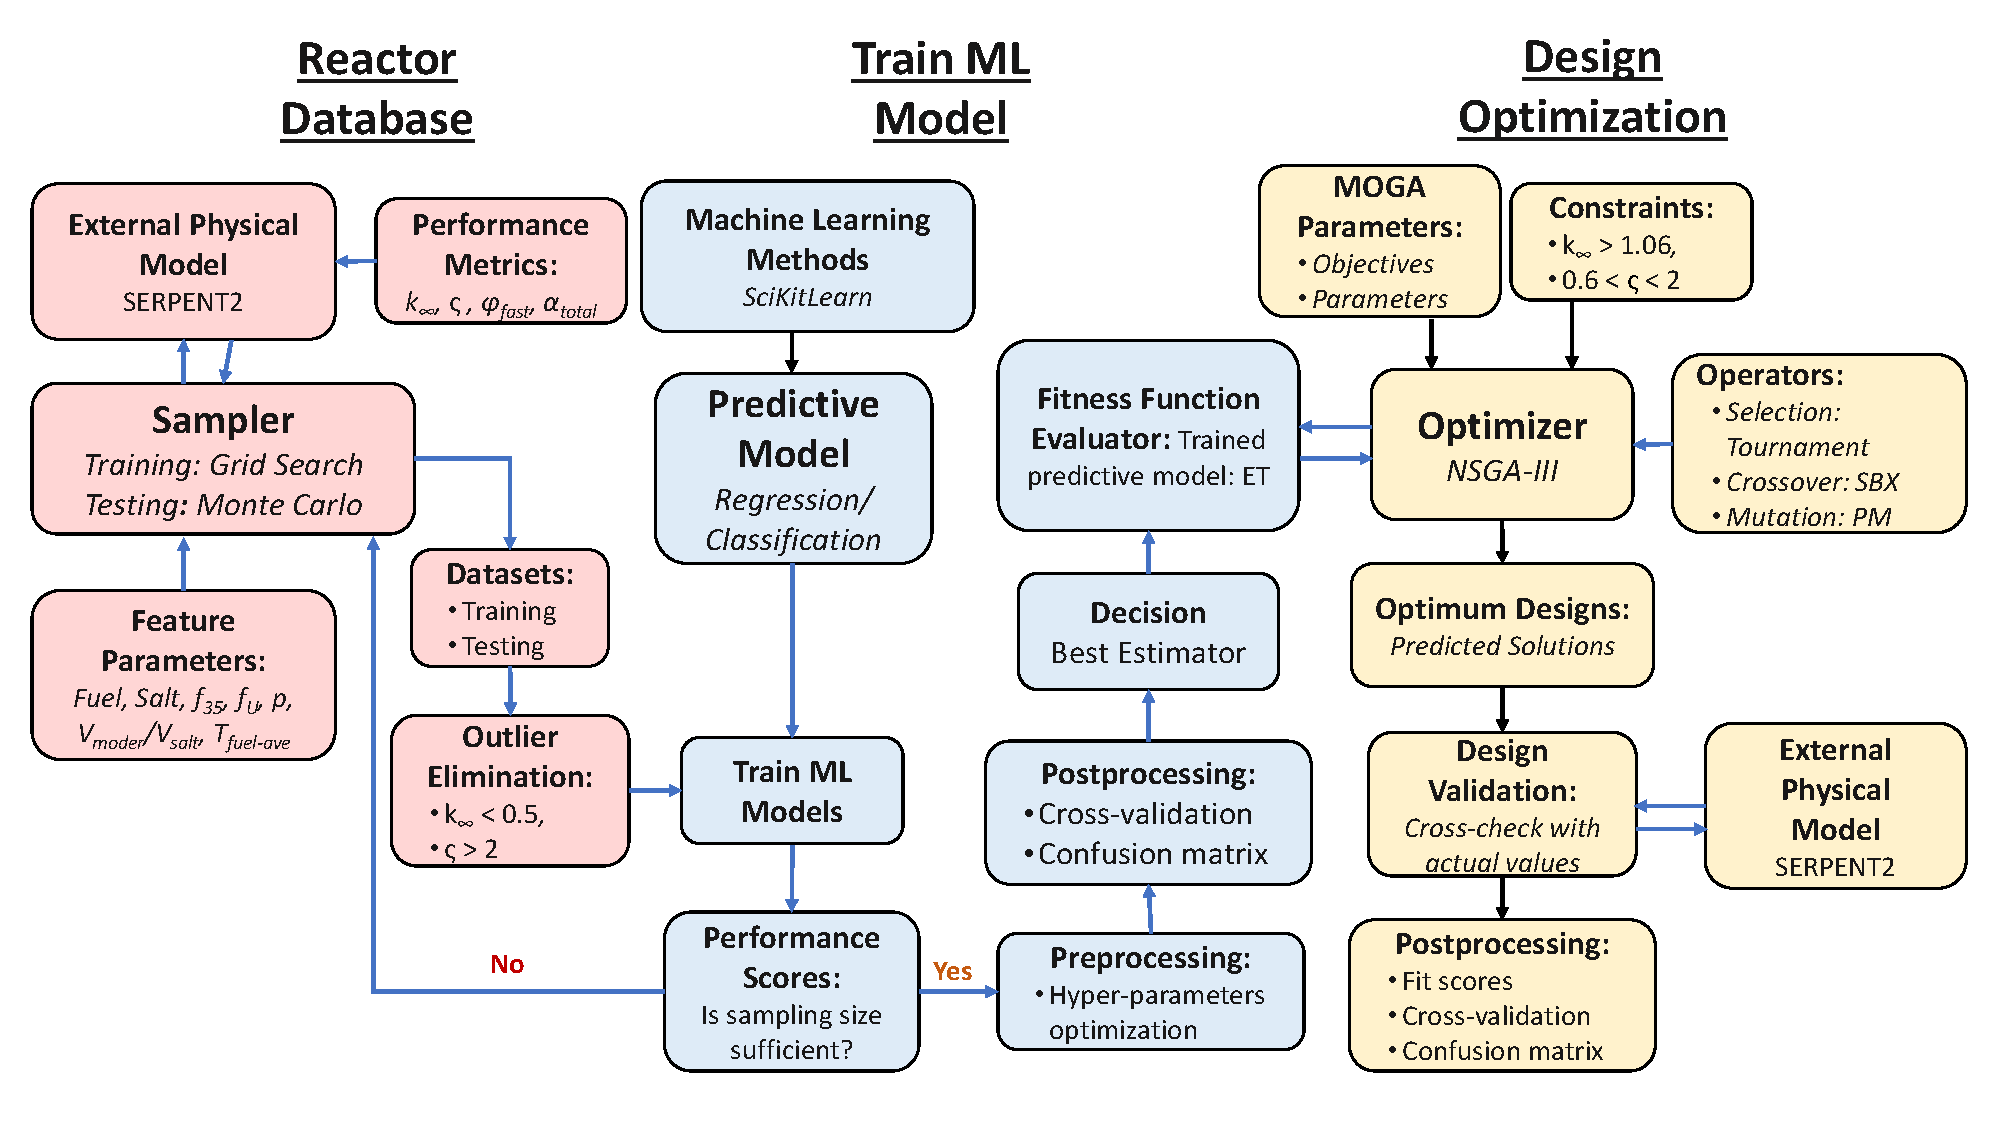
\includegraphics[trim = 0 20 0 20, clip,
    	width=\textwidth]{images/computational_flowchart.pdf}
    	\caption{Computational flowchart of the Plankton code}
    	\label{fig:flowchart}
    \end{figure}

\subsection{Plankton}

\subsubsection{Database Generation}

    \DIFdelbegin \DIFdel{The database generation is the }\DIFdelend \DIFaddbegin \DIFadd{Database generation is a }\DIFaddend step in which samplings in datasets are created and, training and \DIFdelbegin \DIFdel{testing }\DIFdelend \DIFaddbegin \DIFadd{test }\DIFaddend datasets are produced based on two distinctive sampling \DIFdelbegin \DIFdel{strategy}\DIFdelend \DIFaddbegin \DIFadd{strategies}\DIFaddend , Grid sampling and Monte Carlo.

    The grid sampling strategy, the simplest exploration approach to explore an uncertain domain, was used to obtain the training dataset. It constructs an N-dimensional grid in which each dimension accounts for a single feature parameter. \DIFaddbegin \DIFadd{Also, each dimension is discretized with the step values (the rightmost column in Table 3) into equally-spaced intervals between its upper and lower bounds. }\DIFaddend A sample in \DIFdelbegin \DIFdel{the dataset represents }\DIFdelend \DIFaddbegin \DIFadd{a dataset is represented by }\DIFaddend a specific node in the grid \DIFaddbegin \DIFadd{system}\DIFaddend .

    \DIFdelbegin \DIFdel{In contrast to }\DIFdelend \DIFaddbegin \DIFadd{Unlike }\DIFaddend the grid strategy, \DIFdelbegin \DIFdel{a }\DIFdelend \DIFaddbegin \DIFadd{the }\DIFaddend test dataset was generated by the Monte Carlo technique\DIFdelbegin \DIFdel{in which }\DIFdelend \DIFaddbegin \DIFadd{, where }\DIFaddend the value of each variable is randomly determined between \DIFdelbegin \DIFdel{the }\DIFdelend \DIFaddbegin \DIFadd{its }\DIFaddend lower and upper limits.
\DIFaddbegin 

    \DIFaddend As the size of \DIFdelbegin \DIFdel{samplings }\DIFdelend \DIFaddbegin \DIFadd{the training dataset }\DIFaddend has a significant effect on \DIFdelbegin \DIFdel{fitting scoresof the training data, the determination }\DIFdelend \DIFaddbegin \DIFadd{performance scores, the }\DIFaddend criteria for the \DIFdelbegin \DIFdel{size of datasets were explicitly defined in }\DIFdelend \DIFaddbegin \DIFadd{required size were discussed in detail in }\DIFaddend the learning curve section. \DIFdelbegin \DIFdel{Therefore, the estimation of the optimum training sample size is performed by
the ' learning $\_$curve' tool }\DIFdelend \DIFaddbegin \DIFadd{For this, we examined estimators' learning curves }\DIFaddend in conjunction with \DIFdelbegin \DIFdel{'ShuffleSplit'}\DIFdelend \DIFaddbegin \DIFadd{the cross-validation splitting strategy}\DIFaddend , which examines the change in the validation and training score of an estimator for which the number of training samples varies.

    Computational steps \DIFdelbegin \DIFdel{performed in }\DIFdelend \DIFaddbegin \DIFadd{followed in the }\DIFaddend database generation phase \DIFaddbegin \DIFadd{are as follows}\DIFaddend :
    \begin{itemize}
        \item Initialize \DIFdelbegin \DIFdel{the }\DIFdelend feature parameters, properties of which are given in Table~\ref{table:features}, for the grid search technique and Monte Carlo method.
        \item Prepare \DIFdelbegin \DIFdel{the }\DIFdelend input files for the reactor physics code for neutron transport calculation and simulate each sample in \DIFdelbegin \DIFdel{training and testing }\DIFdelend \DIFaddbegin \DIFadd{the training and test }\DIFaddend datasets.
        \item Calculate \DIFdelbegin \DIFdel{the }\DIFdelend performance metrics and extract them from the code output.
        \item Supply the prepared reactor database, a set of training/\DIFdelbegin \DIFdel{testing samples which }\DIFdelend \DIFaddbegin \DIFadd{test samples that }\DIFaddend comprise the feature parameters with \DIFaddbegin \DIFadd{the }\DIFaddend corresponding performance metrics, to the machine learning phase.
    \end{itemize}

\subsubsection{Machine Learning}

    In this part, we \DIFaddbegin \DIFadd{employed regression analysis for the estimation of performance metrics and considered classification analysis, which differs from the regression part in terms of feature parameters, to determine classes of a design. We intended to separately use both methods within the scope of this study, but we are also planning to integrate them for the determination of optimal designs for future work. We }\DIFaddend scoped out various regressors and classifiers from \gls{ML} methods \DIFdelbegin \DIFdel{with }\DIFdelend \DIFaddbegin \DIFadd{within }\DIFaddend the scikit-learn python package \cite{Ped2011} \DIFaddbegin \DIFadd{in order for the assessment of the best performing estimator(s)}\DIFaddend . Table~\ref{table:AImethods} lists \DIFaddbegin \DIFadd{the }\DIFaddend \gls{ML} methods including semi-supervised and supervised methods such as \gls{NN}, ensemble, linear, \gls{SVM}, \DIFdelbegin \DIFdel{decision tree, naive bayes, and neighbor-based }\DIFdelend \DIFaddbegin \gls{DTs}\DIFadd{, }\gls{NB}\DIFadd{, and nearest neighbours }\DIFaddend methods. Because there is more than one performance metric, \DIFdelbegin \DIFdel{the estimators need }\DIFdelend \DIFaddbegin \DIFadd{estimators require }\DIFaddend a built-in or external multi-class/multi-label support. We\DIFdelbegin \DIFdel{therefore }\DIFdelend \DIFaddbegin \DIFadd{, therefore, }\DIFaddend used the multi-target multi-output method in regression and multi-label multi-output method in classification when necessary. \DIFdelbegin \DIFdel{In this context, either 'MultiOutput' or 'OneVsRest' tools (e.g., for
}%DIFDELCMD < \gls{SV} %%%
\DIFdel{classifier) were utilized. }\DIFdelend We performed a comprehensive performance assessment by examining various regression and classification metrics given in Table~\ref{table:MLmetrics}. Prior to regression/classification analyses, we standardized our datasets by \DIFdelbegin \DIFdel{the MinMaxScaler scaler that scales }\DIFdelend \DIFaddbegin \DIFadd{scaling }\DIFaddend each feature parameter between zero and one.

    \DIFdelbegin \DIFdel{For the optimization of the hyper-parameters of the }\DIFdelend \DIFaddbegin \DIFadd{We evaluated the performances of regressors by cross-validation plots and   the performance of classifiers by confusion matrices. Cross-validation is for the visualization of prediction errors whereas confusion matrix is a table that contains all the defined classes in both the horizontal and vertical directions. In a confusion matrix, predicted outputs are listed along the top of a table whereas actual values are listed on the left-hand side column of the table. Anything on the primary diagonal is correctly predicted values. Values above and below the primary diagonal are incorrectly predicted labels called false negative and false possitive.
}

    \DIFadd{For the optimization of hyperparameters of }\DIFaddend estimators, we performed an    exhaustive search over specified parameter values \DIFdelbegin \DIFdel{using GridSearchCV within the
scikit-learn module }\DIFdelend to further improve the scores of estimators. \DIFaddbegin \DIFadd{The scoring parameters were set to f1 samples in classification and }\gls{R2} \DIFadd{in regression.
}\DIFaddend 

    Computational steps \DIFdelbegin \DIFdel{performed in }\DIFdelend \DIFaddbegin \DIFadd{followed in the }\DIFaddend machine learning phase \DIFaddbegin \DIFadd{are as follows}\DIFaddend :
    \begin{itemize}
    	\item As a starting point, use diverse \gls{ML} methods \DIFdelbegin \DIFdel{, }\DIFdelend listed in Table~\ref{table:AImethods} \DIFdelbegin \DIFdel{, }\DIFdelend from the scikit-learn tool.
    	\item With the default settings of \DIFdelbegin \DIFdel{hyper-parameters, assess the }\DIFdelend \DIFaddbegin \DIFadd{hyperparameters, assess }\DIFaddend potential estimators to be used in training just by looking into their fit \DIFdelbegin \DIFdel{performances
	}\DIFdelend \DIFaddbegin \DIFadd{scores }\DIFaddend and exclude the worst ones from the list of the potential estimators.
    	\item Analyze \DIFdelbegin \DIFdel{the }\DIFdelend learning curves of the selected estimators to understand the optimal \DIFdelbegin \DIFdel{sample size required for a }\DIFdelend \DIFaddbegin \DIFadd{size of a training dataset required for }\DIFaddend high-quality training.
    	\item Make a \DIFdelbegin \DIFdel{hyper-parameter }\DIFdelend \DIFaddbegin \DIFadd{hyperparameter }\DIFaddend optimization for the selected estimators to further improve the \DIFdelbegin \DIFdel{estimators' scores }\DIFdelend \DIFaddbegin \DIFadd{scores of the estimators}\DIFaddend .
    	\item Eliminate \DIFdelbegin \DIFdel{the outliers for which }\DIFdelend \DIFaddbegin \DIFadd{outliers according to }\DIFaddend the performance metrics \DIFdelbegin \DIFdel{which seem
	}\DIFdelend \DIFaddbegin \DIFadd{of the estimators seemingly }\DIFaddend impracticable from the viewpoint of designing a reactor and \DIFdelbegin \DIFdel{are }\DIFdelend out of interest \DIFdelbegin \DIFdel{,
	}\DIFdelend \DIFaddbegin \DIFadd{in order }\DIFaddend to further improve the estimators' scores \DIFdelbegin \DIFdel{, focusing on only the }\DIFdelend \DIFaddbegin \DIFadd{and focus on only }\DIFaddend feasible solution domain.
    	\item Select the best estimator(s) according to \DIFdelbegin \DIFdel{their fitting scores }\DIFdelend \DIFaddbegin \DIFadd{the fit scores of the estimators}\DIFaddend .
    	\item \DIFdelbegin \DIFdel{For better understanding of }\DIFdelend \DIFaddbegin \DIFadd{To better understand }\DIFaddend the selected estimators' capability, get the final scores of the estimators, cross-validate the results of the	regressors, and draw confusion matrices of the classifiers.
    	\item Supply the best estimator(s) (along with the optimized \DIFdelbegin \DIFdel{hyper-parameters}\DIFdelend \DIFaddbegin \DIFadd{hyperparameters}\DIFaddend ) to the design optimization phase to predict the performance	metrics of \DIFdelbegin \DIFdel{the }\DIFdelend objective functions.
    \end{itemize}

%%%%%%%%%%%%%%%%%%%%%%%%%%%%%%%%%%%%%%%%
    \begin{table}[ht!]
    	\centering
    	\caption{Examined \gls{ML} methods \cite{Ped2011}}
    	\begin{tabular}{ll}
    		\hline
    		\textbf{Method} & \textbf{Estimator}    \\ \hline
    		\DIFdelbeginFL \DIFdelFL{Ensemble  }\DIFdelendFL \DIFaddbeginFL \DIFaddFL{ensemble  }\DIFaddendFL & \gls{RF}, \DIFdelbeginFL \DIFdelFL{Bagging (B)  }\DIFdelendFL \DIFaddbeginFL \gls{B}  \DIFaddendFL \\
    		& \DIFdelbeginFL \DIFdelFL{AdaBoost (AB)}\DIFdelendFL \DIFaddbeginFL \gls{AB}\DIFaddendFL , \gls{ET} \\
    		& \DIFdelbeginFL \DIFdelFL{GradientBoosting (GB)   }\DIFdelendFL \DIFaddbeginFL \gls{GB}   \DIFaddendFL \\
    		\DIFdelbeginFL \DIFdelFL{Linear    }\DIFdelendFL \DIFaddbeginFL \DIFaddFL{linear    }\DIFaddendFL &\DIFdelbeginFL \DIFdelFL{ElasticNet (EN), Perceptron (P), Ridge (R) }\DIFdelendFL \DIFaddbeginFL \gls{EN}\DIFaddFL{, }\gls{P}\DIFaddFL{, }\gls{R} \DIFaddendFL \\
    		& \DIFdelbeginFL \DIFdelFL{StochasticGradientDescent (SGD)  }\DIFdelendFL \DIFaddbeginFL \gls{SGD}  \DIFaddendFL \\
    		& \DIFdelbeginFL \DIFdelFL{Lasso (L), LassoLars (LL), Logistic (Log) }\DIFdelendFL \DIFaddbeginFL \gls{L}\DIFaddFL{, }\gls{LL}\DIFaddFL{, }\gls{Log} \DIFaddendFL \\
    		\DIFdelbeginFL \DIFdelFL{Naive Bayes     }\DIFdelendFL \DIFaddbeginFL \gls{NB}  \DIFaddendFL & \DIFdelbeginFL \DIFdelFL{GaussianNB (GNB), BernoulliNB (BNB)}\DIFdelendFL \DIFaddbeginFL \gls{GNB}\DIFaddFL{, }\gls{BNB}\DIFaddendFL \\
    		\DIFdelbeginFL \DIFdelFL{Neighbor-Based  }\DIFdelendFL \DIFaddbeginFL \DIFaddFL{nearest neighbors  }\DIFaddendFL & \gls{KN} \\
    		\gls{SVM} & \DIFdelbeginFL %DIFDELCMD < \gls{SV} %%%
\DIFdelendFL \DIFaddbeginFL \gls{SVM} \DIFaddendFL \\
    		\gls{NN}  & \gls{MLP} \\
    		\DIFdelbeginFL %DIFDELCMD < \gls{DT}  %%%
\DIFdelendFL \DIFaddbeginFL \gls{DTs}  \DIFaddendFL & \gls{DT}  \\
    		\DIFdelbeginFL \DIFdelFL{Semi-Supervised }\DIFdelendFL \DIFaddbeginFL \DIFaddFL{semi-supervised }\DIFaddendFL & \DIFdelbeginFL \DIFdelFL{LabelPropagation (LP) }\DIFdelendFL \DIFaddbeginFL \gls{LP} \DIFaddendFL \\ \hline
    	\end{tabular}
    	\label{table:AImethods}
    \end{table}
    %%%%%%%%%%%%%%%%%%%%%%%%%%%%%%%%%%%%%%%%
    \begin{table}[ht!]
    	\centering
    	\caption{Metrics for \DIFaddbeginFL \DIFaddFL{the }\DIFaddendFL performance assessment of estimators \cite{Ped2011}}
    	\DIFdelbeginFL %DIFDELCMD < \resizebox{\textwidth}{!}{%
%DIFDELCMD < 		\begin{tabular}{ll}
%DIFDELCMD < 			\hline
%DIFDELCMD < 			\textbf{Regression}                  & \textbf{Classification}                  \\ \hline
%DIFDELCMD < 			fit score (fit$\_$score)             & fit score (fit$\_$score)                 \\
%DIFDELCMD < 			mean square error (MSE)              & average precision (AP)                   \\
%DIFDELCMD < 			mean absolute error (MAE)            & ranking-based average precision (LRAPS)  \\
%DIFDELCMD < 			explained variance regression (EVR)  & label ranking loss (LRL)                 \\
%DIFDELCMD < 			coefficient of determination (R$^2$) & average Hamming loss (HL)                \\
%DIFDELCMD < 			& computed area under the receiver         \\
%DIFDELCMD < 			& operating characteristic curve (ROC-AUC) \\ \hline
%DIFDELCMD < 	\end{tabular}}
%DIFDELCMD < 	%%%
\DIFdelendFL \DIFaddbeginFL \resizebox{\textwidth}{!}{%
    		\begin{tabular}{p{0.5\linewidth} p{0.5\linewidth}}
    		\hline
    		    \textbf{Regression} & \textbf{Classification} \\
    		\hline
    		    fit score: $\in$ [0, 1], best score: 1         &
                fit score: $\in$ [0, 1], best score: 1              \\
    		    \gls{MSE}, best score: 0           &
                \gls{AP}: $\in$ [0, 1], best score: 1              \\
    		    \gls{MAE}, best score: 0           &
                \gls{LRAPS}: $\in$ [0, 1], best score: 1           \\
    		    \gls{EVR}: $\in$ [0, 1], best score: 1          &
                \gls{LRL}: $\in$ [0, 1], best score: 0             \\
    		    \gls{R2}: $\in$ [0, 1], best score: 1          &
                \gls{HL}: $\in$ [0, 1], best score: 0              \\
    		  & \gls{ROCAUC}: $\in$ [0, 1], best score: 1           \\
    		\hline
    		\end{tabular}}
    	\DIFaddendFL \label{table:MLmetrics}
    \end{table}
%%%%%%%%%%%%%%%%%%%%%%%%%%%%%%%%%%%%%%%%

\subsubsection{Design Optimization}

    In the final stage of the channel design, we aimed at finding \DIFdelbegin \DIFdel{the }\DIFdelend optimal designs. We implemented a multi-variable multi-objective evolutionary algorithm \DIFaddbegin \DIFadd{appropriate to design space's structure which manifests multimodal rather than unimodal}\DIFaddend . We selected this method because optimization methods such as gradient-based or non-linear least-square do not accept discrete and non-numeric variables\DIFdelbegin \DIFdel{. We
opted for an optimization method appropriate to the problem's behavior which
manifests a convex structure rather than a linear relationship.
}\DIFdelend \DIFaddbegin \DIFadd{, and do not work well in non-convex design spaces.
}\DIFaddend 

    We defined the number of generations as a convergence stopping criterion. After finding the \DIFdelbegin \DIFdel{optimum designswith Plankton's ML methods}\DIFdelend \DIFaddbegin \DIFadd{optimal designs}\DIFaddend , we rerun Serpent tool \DIFdelbegin \DIFdel{with the optimal design }\DIFdelend \DIFaddbegin \DIFadd{\mbox{%DIFAUXCMD
\cite{Lep2014} }\hspace{0pt}%DIFAUXCMD
with their }\DIFaddend feature parameters to crosscheck the solutions. \DIFdelbegin \DIFdel{Thus, we
performed additional neutron transport calculations for the optimal designs via
the reactor physics code, used to generate the reactor database. Acceptance
criteria for the }\DIFdelend \DIFaddbegin \DIFadd{The acceptance criterion for the }\DIFaddend accuracy of the optimal designs was selected as:
    \begin{eqnarray}\label{Eq0}
    \dfrac{x_{i,a}-x_{i,p}}{x_{i,a}} \leq 5%DIF < 
\DIFaddbegin \DIFadd{\%
    }\DIFaddend \end{eqnarray}
    where $x_{i,a}$ is the actual value of i$th$ metric and $x_{i,p}$ is the predicted value of i$th$ metric.

    Computational steps \DIFdelbegin \DIFdel{performed in }\DIFdelend \DIFaddbegin \DIFadd{followed in the }\DIFaddend design optimization phase \DIFaddbegin \DIFadd{are as follows}\DIFaddend :
    \begin{itemize}
    	\item \DIFdelbegin \DIFdel{Initialize the }\DIFdelend \DIFaddbegin \DIFadd{Specify an optimization tool (}\DIFaddend \gls{MOGA} \DIFdelbegin \DIFdel{parameters including }\DIFdelend \DIFaddbegin \DIFadd{method) consistent with the structure of the feature parameters and the problem at hand.
        }\item \DIFadd{Determine tool's parameters such as }\DIFaddend decision variables, operators, number of generations, \DIFaddbegin \DIFadd{and }\DIFaddend initial population size\DIFdelbegin \DIFdel{, crossover rate
	and mutation ratio}\DIFdelend .
    	\item Define \DIFdelbegin \DIFdel{the }\DIFdelend constraints for the performance metrics \DIFdelbegin \DIFdel{which would
	}\DIFdelend \DIFaddbegin \DIFadd{to }\DIFaddend eliminate undesired designs.
    	\item \DIFdelbegin \DIFdel{Use a }%DIFDELCMD < \gls{GA} %%%
\DIFdel{method, which are naturally
	limited by the problem, consistent with the structure of the feature parameters.
	}%DIFDELCMD < \item %%%
\item%DIFAUXCMD
\DIFdel{Couple the estimator (s) to the }%DIFDELCMD < \gls{GA} %%%
\DIFdel{method to calculate the
	}\DIFdelend \DIFaddbegin \DIFadd{Integrate the optimizer with the best performing estimator (in place of reactor physics code) to evaluate the }\DIFaddend performance metrics of \DIFdelbegin \DIFdel{the objective functions, without running a reactor physics
	code}\DIFdelend \DIFaddbegin \DIFadd{objective functions}\DIFaddend .
    	\item Iterate this \gls{ML}-\gls{GA} coupled system until either the constraints are met or the solutions are converged to one of the predefined criteria.
    	\item \DIFdelbegin \DIFdel{Verify the pareto-front }\DIFdelend \DIFaddbegin \DIFadd{Validate Pareto-front }\DIFaddend (predicted) solutions \DIFdelbegin \DIFdel{by calculating actual values }\DIFdelend \DIFaddbegin \DIFadd{with actual values (with additional Serpent simulation)}\DIFaddend .
    \end{itemize}

\subsection{Channel Design with Plankton}

\subsubsection{Design Parameters}

    We applied the suggested method to a single fuel channel \gls{MSR} geometry with square unit cell approximation to use in a basic geometry with the least number of feature parameters and performance metrics. An illustration of the channel geometry is shown in Figure~\ref{fig:channel}. \DIFaddbegin \DIFadd{In the figure, $p$ is the pitch length, $T_{in}$ and $T_{out}$ are inlet and outlet temperatures, $v_{salt}$ is the velocity of fuel-salt, $L$ is the channel length, $R_f$ is the radius of the fuel-salt channel and $q_{channel}$ is the total heat generation in the channel. }\DIFaddend Feature parameters describing \DIFdelbegin \DIFdel{the
}\DIFdelend material and geometry properties of the \DIFdelbegin \DIFdel{single }\DIFdelend channel were selected as fuel type, salt type, $^{235}$U fraction ($f_{35}$) in U, U fraction ($f_{U}$) in heavy metal, channel-to-channel pitch length ($p$), moderator-to-salt volume ratio ($\xi$), and average fuel-salt temperature ($T_{ave}$) along the channel. We varied \DIFdelbegin \DIFdel{the }\DIFdelend \DIFaddbegin \DIFadd{these }\DIFaddend variables between upper and lower bounds described in Table~\ref{table:features}. The $^{235}$U fraction in U was limited to 20 wt.\% which is the maximum limit for \gls{HALEU}. For the fuel types other than U fuel type, U content in heavy metal varies from 10 to 90 wt.\%. The maximum $p$, based on \gls{ORNL}'s \gls{MSRE} design \DIFaddbegin \DIFadd{\mbox{%DIFAUXCMD
\cite{robertson1971}}\hspace{0pt}%DIFAUXCMD
}\DIFaddend , was set to 16 cm. \DIFdelbegin \DIFdel{The $\xi$ variable
was calculated from }\DIFdelend \DIFaddbegin \DIFadd{From }\DIFaddend the ratio of pitch \DIFdelbegin \DIFdel{to fuel salt radius between }\DIFdelend \DIFaddbegin \DIFadd{length to fuel-salt channel radius ($p/R_{f}$), the $\xi$ variable was calculated and found in the range of }\DIFaddend 0.274 (\DIFdelbegin \DIFdel{p/D$_{fuel}$ }\DIFdelend \DIFaddbegin \DIFadd{$p/R_{f}$ }\DIFaddend = \DIFdelbegin \DIFdel{1}\DIFdelend \DIFaddbegin \DIFadd{0.5}\DIFaddend ) and 10.46 (\DIFdelbegin \DIFdel{p/D$_{fuel}$ }\DIFdelend \DIFaddbegin \DIFadd{$p/R_{f}$ }\DIFaddend = \DIFdelbegin \DIFdel{3}\DIFdelend \DIFaddbegin \DIFadd{1.5}\DIFaddend ).

    We studied three different fuel types, U, U-Th\DIFaddbegin \DIFadd{, }\DIFaddend and U-Pu in this work. Th in U-Th contains only $^{232}$Th isotope whereas Pu in U-Pu comes from the \DIFdelbegin \DIFdel{weapon-grade
}\DIFdelend \DIFaddbegin \DIFadd{weapons-grade }\DIFaddend Pu constituting the following isotopes: $^{238}$Pu (0.05 at.\%), $^{239}$Pu (94.3 at.\%), $^{240}$Pu (5 at.\%), $^{241}$Pu (0.6 at.\%) and $^{242}$Pu (0.05 at.\%). It is assumed that there is no $^{234}$U in U as a parasitic absorber.

    We examined three types of different salts widely used in prototype reactors by various companies (Terrestrial Energy, Terrapower, Thorcon, etc.): LiF-BeF$_2$, NaF-BeF$_2$, and NaCl. The upper value of \DIFaddbegin \DIFadd{the }\DIFaddend average fuel-salt temperature ($T_{ave}$) is set to 1200 K while its base temperature used to calculate the total feedback coefficient of reactivity is 900 K. As the temperature is the main driver for \DIFdelbegin \DIFdel{fuel salt }\DIFdelend \DIFaddbegin \DIFadd{fuel-salt }\DIFaddend density and Doppler effect \DIFdelbegin \DIFdel{on }\DIFdelend \DIFaddbegin \DIFadd{of }\DIFaddend feedback, salt density variation with the $T_{ave}$ was taken into account based on the reports \cite{Janz1988, Jerden2019}.

    \DIFdelbegin \DIFdel{The }\DIFdelend \DIFaddbegin \DIFadd{In the regression analysis, the }\DIFaddend most critical performance metrics are \DIFdelbegin \DIFdel{the }\DIFdelend \DIFaddbegin \DIFadd{selected as }\DIFaddend infinite multiplication factor ($k_{\infty}$), conversion ratio ($\varsigma$), fast flux ($\phi_{fast}$) incident on the graphite moderator\DIFaddbegin \DIFadd{, }\DIFaddend and total feedback coefficient (${\alpha_{total}}$). \DIFdelbegin \DIFdel{However, ${\alpha_{total}}$ was not considered as performance metrics in ML phase as it can be calculated }\DIFdelend \DIFaddbegin \DIFadd{But, we did not include the ${\alpha_{total}}$ as a performance metric since this metric caused huge errors in scores, probably due to zero values at 900 K. Yet, we }\DIFaddend promptly and accurately \DIFaddbegin \DIFadd{calculated it }\DIFaddend from Eq. \protect\ref{Eq1} using $k_{\infty}$ \DIFdelbegin \DIFdel{, thus being calculated }\DIFdelend at the end of the design optimization phase.

    In \DIFaddbegin \DIFadd{the }\DIFaddend classification analysis, \DIFdelbegin \DIFdel{a channel design was labeled }\DIFdelend \DIFaddbegin \DIFadd{the ${\alpha_{total}}$ metric did not cause any trouble so that we were able to use it. We labeled the single channel design }\DIFaddend with different labels according to its spectrum, type, criticality condition\DIFaddbegin \DIFadd{, }\DIFaddend and positive or \DIFaddbegin \DIFadd{the }\DIFaddend negative sign of the feedback coefficient. Accordingly, we addressed any channel design as breeder type when $\varsigma \geq 1.0$, as fast spectrum when \gls{EALF} $\geq 1eV$, as supercritical condition when $k_{\infty} \geq 1.0$, and as positive feedback when ${\alpha_{total}} \geq 0.0$. For the opposite of these conditions, the design is labeled as burner type, thermal spectrum, sub-critical condition, and negative feedback, respectively.

    Associated with the channel design, we made the following approximations, simplifications\DIFaddbegin \DIFadd{, }\DIFaddend and approaches involved in the model/method development:
    \begin{itemize}
    	\item The unit cell approximation \DIFdelbegin \DIFdel{with }\DIFdelend \DIFaddbegin \DIFadd{in }\DIFaddend a square lattice \DIFaddbegin \DIFadd{geometry }\DIFaddend was chosen to represent the single channel geometry. It is an effective geometry structure for periodicity.
    	\item The fuel-salt \DIFdelbegin \DIFdel{is }\DIFdelend \DIFaddbegin \DIFadd{was }\DIFaddend assumed to be stationary, by neglecting thermal-hydraulic effects such as delayed neutron precursor movement.
    	\item Calculations were performed for initial fuel loading assuming fresh fuel.
    	\item \DIFdelbegin \DIFdel{Total }\DIFdelend \DIFaddbegin \DIFadd{The total }\DIFaddend heat generation	rate along the channel \DIFdelbegin \DIFdel{is }\DIFdelend \DIFaddbegin \DIFadd{was }\DIFaddend expressed in terms of an arithmetic average of the inlet and outlet temperatures, i.e., $T_{ave}$ = ($T_{in}$+$T_{out}$)/2, thereby \DIFdelbegin \DIFdel{, }\DIFdelend making the design independent from the length	of the channel.
    \end{itemize}

    Using these approximations, we eliminated four interdependent variables: inlet and outlet temperatures, heat generation rate, and channel length\DIFdelbegin \DIFdel{, to the
average temperature definition}\DIFdelend . We reduced the total number of feature parameters from eleven to seven parameters.

%%%%%%%%%%%%%%%%%%%%%%%%%%%%%%%%%%%%%%%%
    \begin{figure}[ht!]
    	\centering
    	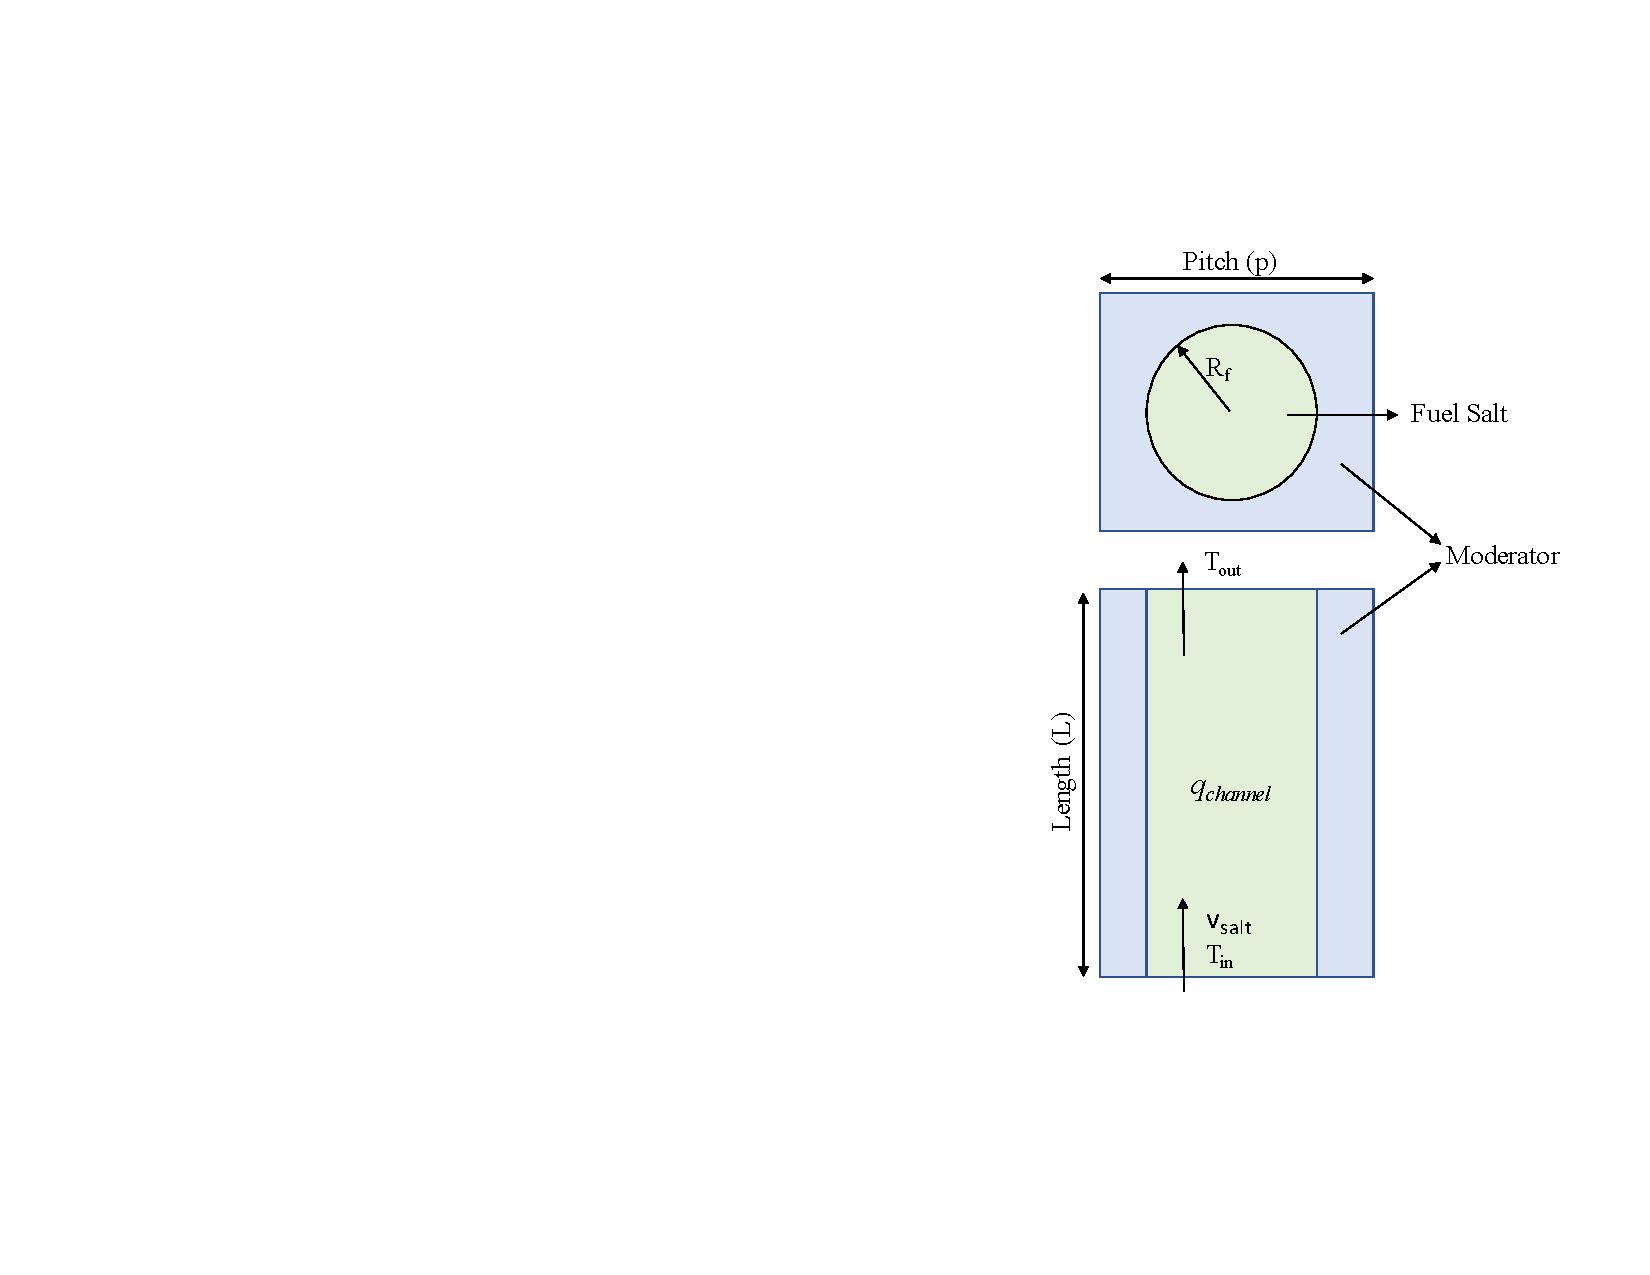
\includegraphics[trim=500 140 0 100, clip,
    	scale=0.6]{images/single_channel.pdf}
    	\caption{Single fuel channel representation\DIFaddbeginFL \DIFaddFL{.}\DIFaddendFL }
    	\label{fig:channel}
    \end{figure}
%%%%%%%%%%%%%%%%%%%%%%%%%%%%%%%%%%%%%%%%
    \begin{table}[ht!]
    	\centering
    	\caption{Feature parameters for database generation}
    	\begin{tabular}{lllll}
    		\hline
    		\textbf{Variable} & \textbf{Distribution} & \textbf{Material types} & 		& \textbf{Steps} \\ \hline
    		Fuel Type & Discrete   & U, U-Th, U-Pu & & 3 \\
    		Salt Type & Discrete   & LiF-BeF$_2$, NaCl, & NaF-BeF$_2$  & 3 \\
    		&  & \textbf{Lower value} &\textbf{Upper value} &  \\
    		$f_{35}$  & Continuous  & 1 wt.\%   & 20 wt.\% & 10 \\
    		$f_{U}$   & Continuous  & 10 wt.\%  & 90 wt.\% & 9 \\
    		$p$       & Continuous  & 1 cm      & 16 cm & 10 \\
    		$\xi$     & Continuous  & 0.274 & 10.46 & 10 \\
    		$T_{ave}$ & Continuous  & 900 K     & 1200 K & 5 \\ \hline
    	\end{tabular}
    	\label{table:features}
    \end{table}
%%%%%%%%%%%%%%%%%%%%%%%%%%%%%%%%%%%%%%%%

\subsubsection{Optimization Parameters}

    We used the \gls{NSGAIII} \cite{deb2014, jain2014} from the pymoo tool \cite{pymoo2020} as an optimizer with the \gls{SBX} and \gls{PM} operators. The population size and number of generations were set to 150 and 5000, respectively. \DIFdelbegin \DIFdel{Tournament }\DIFdelend \DIFaddbegin \DIFadd{The tournament }\DIFaddend selection, in which a set of chromosomes are selected randomly and then the fittest chromosomes are selected for further operation, was employed to select the fittest candidates from the current generation.

    Several independent constraints imposed by the basic requisites of a \gls{MSR} design were implemented to the solution objectives in \DIFdelbegin \DIFdel{accordance with the references \mbox{%DIFAUXCMD
\cite{rykhlevskii2019, betzler2017, ashraf2019} }\hspace{0pt}%DIFAUXCMD
}\DIFdelend \DIFaddbegin \DIFadd{line with the given references \mbox{%DIFAUXCMD
\cite{robertson1971, rykhlevskii2019, betzler2017, ashraf2019} }\hspace{0pt}%DIFAUXCMD
}\DIFaddend in the following way: \DIFaddbegin \DIFadd{We searched for }\DIFaddend $k_{\infty}$ \DIFdelbegin \DIFdel{is }\DIFdelend greater than 1.06 to make up for neutron leakage\DIFdelbegin \DIFdel{; }\DIFdelend \DIFaddbegin \DIFadd{. Despite the MSRs typically have a conversion ratio of around 1.0, }\DIFaddend $\varsigma$ \DIFdelbegin \DIFdel{is
}\DIFdelend \DIFaddbegin \DIFadd{was chosen as }\DIFaddend higher than 0.6 \DIFdelbegin \DIFdel{; and }\DIFdelend \DIFaddbegin \DIFadd{to include as many designs as into the optimization process. As there is no reported constraints on }\DIFaddend $\phi_{fast}$\DIFaddbegin \DIFadd{, we simply assumed $\phi_{fast}$ }\DIFaddend per source neutron on graphite \DIFdelbegin \DIFdel{in which }\DIFdelend \DIFaddbegin \DIFadd{to be lower than half (50) of what }\DIFaddend the maximum value \DIFdelbegin \DIFdel{is calculated to be about 100 is less than 50.
}\DIFdelend \DIFaddbegin \DIFadd{($\sim100$) of the fast flux in the training dataset is.
}\DIFaddend 

    \DIFdelbegin \DIFdel{In the optimizationproblem, the }\DIFdelend \DIFaddbegin \DIFadd{For optimization, }\DIFaddend feature parameters were assigned as decision variables\DIFdelbegin \DIFdel{while the }\DIFdelend \DIFaddbegin \DIFadd{, while }\DIFaddend performance metrics were assigned as solution objectives (or objective functions). The $k_{\infty}$ and $\varsigma$ metrics were maximized while the $\phi_{fast}$ was minimized.

\subsubsection{Neutronic Simulator}

    We employed a Monte Carlo neutron transport tool, Serpent 2 (2.1\DIFdelbegin \DIFdel{.30}\DIFdelend \DIFaddbegin \DIFadd{.31}\DIFaddend ) \cite{Lep2014} to compute \DIFdelbegin \DIFdel{the performance metricsdefined in design parameters
section}\DIFdelend \DIFaddbegin \DIFadd{performance metrics}\DIFaddend . It uses ENDF/B-VII.0 \cite{chadwick2006} as the neutron cross-section library \DIFdelbegin \DIFdel{along with }\DIFdelend \DIFaddbegin \DIFadd{alongside the }\DIFaddend S(${\alpha}$, ${\beta}$) thermal scattering libraries. In the simulator, neutron population per cycle, passive cycle, and active cycle were set to 2000, 50, and 100, respectively, to yield a computational standard error of less than 100 pcm in the $k_{\infty}$. A two-group neutron energy structure for the calculation of $\phi_{fast}$ on the moderator was used\DIFaddbegin \DIFadd{, }\DIFaddend and lower and upper energy boundaries for the fast region were set to 0.625 eV and 20 MeV, respectively. The $k_{\infty}$, $\varsigma$, and $\phi_{fast}$ metrics were directly extracted from the output file whereas ${\alpha_{total}}$ was calculated by Eq. \protect\ref{Eq1}:
    \begin{eqnarray}\label{Eq1}
    \alpha_{total} = \dfrac{\partial\rho}{\partial T} \approx
    \dfrac{\Delta\rho}{\Delta T}=\dfrac{\rho-\rho_b}{T-T_b}
    \end{eqnarray}
    where $\rho$ is the reactivity, $\rho_b$ is the reactivity at the base temperature, $T$ is the temperature, and $T_b$ is the base temperature. However, we purposefully avoided using $\partial \rho /\partial T$ in estimating \DIFdelbegin \DIFdel{/predicting the feedback coefficient as }\DIFdelend \DIFaddbegin \DIFadd{the }\DIFaddend ${\alpha_{total}}$ \DIFaddbegin \DIFadd{since it }\DIFaddend goes to infinity when $T_{ave}$ is very close to the base temperature\DIFdelbegin \DIFdel{, resulting
problematic outputs}\DIFdelend . Instead, we used $\partial k$(mk) and converted to ${\alpha_{total}}$ at the end of the calculations. For the \DIFdelbegin \DIFdel{energy spectrum
classification of the reactor , }\DIFdelend \DIFaddbegin \DIFadd{estimation of reactor spectrum in classification, we used }\DIFaddend the \gls{EALF}  value \DIFdelbegin \DIFdel{extracted from the output
file was used}\DIFdelend \DIFaddbegin \DIFadd{given in the code output}\DIFaddend .

\subsubsection{Datasets}
    In this work, a total training sample size of 285000 and a total test sample
    size of 8000 were used.



	\section{Results}

\subsection{Preselection}
\DIFdelbegin \DIFdel{Performance scores of various estimators elaborated }\DIFdelend \DIFaddbegin

    \DIFadd{For the estimators listed }\DIFaddend in Table~\ref{table:AImethods}\DIFdelbegin \DIFdel{are presented }\DIFdelend \DIFaddbegin \DIFadd{, we presented performance score }\DIFaddend in Table~\ref{table:regression} for \DIFdelbegin \DIFdel{the regression analyses and presented }\DIFdelend \DIFaddbegin \DIFadd{regression analysis and }\DIFaddend in Table~\ref{table:classification} for \DIFdelbegin \DIFdel{the classification analyses}\DIFdelend \DIFaddbegin \DIFadd{classification analysis}\DIFaddend . The results were obtained using the default \DIFdelbegin \DIFdel{hyper-parameters. Each estimator demonstrated its own characteristic behavior
and, }\DIFdelend \DIFaddbegin \DIFadd{hyperparameters. }\DIFaddend \gls{RF}, \gls{ET}, \gls{KN}, \DIFdelbegin %DIFDELCMD < \gls{SV}%%%
\DIFdelend \DIFaddbegin \gls{SVM}\DIFaddend , and \gls{MLP} estimators predicted the performance metrics with significantly higher accuracy than the others. Even without \DIFdelbegin \DIFdel{optimizing the hyper-parameters of the estimators, $R^2$ }\DIFdelend \DIFaddbegin \DIFadd{hyperparameter optimization, }\gls{R2} \DIFaddend scores of these five estimators \DIFdelbegin \DIFdel{range }\DIFdelend \DIFaddbegin \DIFadd{ranged }\DIFaddend from 90 to 98\% for regression and from 92 to 96\% for classification. This implies that the \DIFdelbegin \DIFdel{models trained }\DIFdelend \DIFaddbegin \DIFadd{trained models }\DIFaddend by these estimators will have very low variance. The \gls{ET} regressor most accurately predicted the performance metrics while the \DIFdelbegin %DIFDELCMD < \gls{SV} %%%
\DIFdelend \DIFaddbegin \gls{SVM} \DIFaddend classifier was superior to \DIFdelbegin \DIFdel{other
estimators in classifying the design labels defined as reactor type, spectrum,
criticality and feedback}\DIFdelend \DIFaddbegin \DIFadd{the others in classifying designs}\DIFaddend .

    In general, the linear methods (i.e., \DIFdelbegin \DIFdel{SGD, R, EN, L, LL, P, and Log) yield lower a fit \_score (and thus higher errors ) }\DIFdelend \DIFaddbegin \gls{SGD}\DIFadd{, }\gls{R}\DIFadd{, }\gls{EN}\DIFadd{, }\gls{L}\DIFadd{, }\gls{LL}\DIFadd{, }\gls{P}\DIFadd{, and }\gls{Log}\DIFadd{) yielded lower fit scores and higher errors }\DIFaddend with respect to the non-linear methods such as ensemble, \gls{SVM}, and \gls{ANN}. These results clearly imply that \DIFdelbegin \DIFdel{the
}\DIFdelend linear methods are not quite enough to design a nuclear reactor and thus in predicting its performance metrics. Like \DIFdelbegin \DIFdel{the }\DIFdelend linear methods, the \DIFdelbegin \DIFdel{Naive Bayes
}\DIFdelend \DIFaddbegin \gls{NB} \DIFaddend classification methods such as \DIFdelbegin \DIFdel{GNB and BNB }\DIFdelend \DIFaddbegin \gls{GNB} \DIFadd{and }\gls{BNB} \DIFaddend seem inappropriate due to the suboptimal performance scores. \DIFaddbegin \DIFadd{This is because these methods such as linear and }\gls{NB} \DIFadd{are not sufficient to fit the training dataset (leading to underfitting) into a linear function due to the higher degree interdependencies of our feature parameters. }\DIFaddend In addition to this, the \gls{RF}, \gls{DT}, \DIFdelbegin \DIFdel{B, and AB regressors and classifiers, have }\DIFdelend \DIFaddbegin \gls{B}\DIFadd{, and }\gls{AB} \DIFadd{estimators, gave }\DIFaddend similar results, except for fit score values, as they use the same base estimator (\DIFdelbegin \DIFdel{decision tree}\DIFdelend \DIFaddbegin \gls{DT}\DIFaddend ) in training. Likewise, the \DIFdelbegin \DIFdel{LP classifier produces }\DIFdelend \DIFaddbegin \gls{LP} \DIFadd{classifier produced }\DIFaddend the same results with the \DIFdelbegin %DIFDELCMD < \gls{SV}
%DIFDELCMD < %%%
\DIFdelend \DIFaddbegin \gls{SVM} \DIFaddend classifier due to the use of the same kernel ($rbf$). In \DIFdelbegin \DIFdel{the }\DIFdelend regression analysis, the \gls{ET} regressor has the lowest \gls{MAE} and \gls{MSE} scores while the \DIFdelbegin \DIFdel{R }\DIFdelend \DIFaddbegin \gls{R} \DIFaddend regressor has the highest scores.

    As to the classification, the \DIFdelbegin %DIFDELCMD < \gls{SV}  %%%
\DIFdelend \DIFaddbegin \gls{SVM} \DIFaddend classifier has the lowest \gls{HL} and \gls{LRL} scores while the \DIFdelbegin \DIFdel{Perceptron }\DIFdelend \DIFaddbegin \gls{P} \DIFaddend classifier has the highest scores. \DIFdelbegin \DIFdel{Furthermore}\DIFdelend \DIFaddbegin \DIFadd{Briefly}\DIFaddend , any design can be classified with \DIFdelbegin \DIFdel{a small fraction of }\DIFdelend \DIFaddbegin \DIFadd{high precision ($>$ 95\%) and very few }\DIFaddend incorrectly predicted labels (\DIFaddbegin \DIFadd{false neagtive plus false positive: }\DIFaddend $<$ 5\%)\DIFdelbegin \DIFdel{and a high precision ($>$ 95\%)}\DIFdelend , leading to an opportunity for an accurate prediction of reactor design even without making any regression analysis.

    \DIFdelbegin \DIFdel{From the results of the preselection phase}\DIFdelend \DIFaddbegin \DIFadd{On the whole}\DIFaddend , five estimators (i.e., \gls{RF}, \gls{ET}, \gls{KN}, \DIFdelbegin %DIFDELCMD < \gls{SV}%%%
\DIFdelend \DIFaddbegin \gls{SVM}\DIFaddend , and \gls{MLP}) \DIFdelbegin \DIFdel{satisfying }\DIFdelend \DIFaddbegin \DIFadd{that satisfy }\DIFaddend a score of more than 90\% in \DIFdelbegin \DIFdel{the $R^2$ and fit score values seem }\DIFdelend \DIFaddbegin \gls{R2} \DIFadd{and fit scores appear to be }\DIFaddend suitable for the subsequent stage of \DIFdelbegin \DIFdel{the }\DIFdelend calculations. Among the selected estimators, \DIFdelbegin \DIFdel{despite its worst fit score
value, the }%DIFDELCMD < \gls{SV} %%%
\DIFdelend \DIFaddbegin \DIFadd{the }\gls{SVM} \DIFaddend regressor interestingly shows the second-best performance right after the \gls{ET} regressor \DIFaddbegin \DIFadd{despite its worst fit score}\DIFaddend . In fact, \DIFdelbegin \DIFdel{all }\DIFdelend \DIFaddbegin \DIFadd{as }\DIFaddend the scores of the \DIFdelbegin \DIFdel{five selected
}\DIFdelend \DIFaddbegin \DIFadd{best performing }\DIFaddend estimators are very close to each other\DIFdelbegin \DIFdel{and }\DIFdelend \DIFaddbegin \DIFadd{, }\DIFaddend at this point\DIFaddbegin \DIFadd{, }\DIFaddend it is not easy to distinguish which estimator is \DIFaddbegin \DIFadd{the }\DIFaddend best. Therefore, in the following section, the \DIFaddbegin \DIFadd{current }\DIFaddend scores of these \DIFdelbegin \DIFdel{five }\DIFdelend estimators are further improved by tuning their \DIFdelbegin \DIFdel{hyper-parameters}\DIFdelend \DIFaddbegin \DIFadd{hyperparameters and investigating their learning curves}\DIFaddend .

%%%%%%%%%%%%%%%%%%%%%%%%%%%%%%%%%%%%%%%%
\begin{landscape}
	\begin{table}[ht!]
		\centering
		\caption{Performance scores \DIFdelbeginFL \DIFdelFL{for various }\DIFdelendFL \DIFaddbeginFL \DIFaddFL{of the studied }\DIFaddendFL regression methods}
		\begin{tabular}{l>{\columncolor[gray]{0.9}}l>{\columncolor[gray]{0.9}}
				l>{\columncolor[gray]{0.9}}l>{\columncolor[gray]{0.9}}
				l>{\columncolor[gray]{0.9}}lllllllllllllllllllllllllll}
			\hline
			& \textbf{\gls{RF}} & \textbf{\gls{ET}} & \textbf{\gls{KN}} &
			\textbf{\DIFdelbeginFL %DIFDELCMD < \gls{SV}%%%
\DIFdelendFL \DIFaddbeginFL \gls{SVM}\DIFaddendFL } & \textbf{\gls{MLP}} & \textbf{\gls{DT}} & \textbf{GB} &
			\textbf{B} & \textbf{AB} & \textbf{SGD} & \textbf{R} & \textbf{EN} &
			\textbf{L} & \textbf{LL} \\
			\hline
			fit \DIFdelbeginFL \DIFdelFL{$\_$}\DIFdelendFL score & 1.00 & 1.00 	& 0.99  & 0.96 	& 0.99  & 1.00 & 0.97 & 1.00
			& 0.78	& 0.54 	& 0.73 	& 0.70 	& 0.69 	& 0.55 \\
			EVR  & 0.90 & 0.98 & 0.97 & 0.98 	& 0.95  & 0.90 &
			0.89 & 0.90 & 0.54	& 0.38 & 0.37 & 0.46 & 0.25 & 0.38 \\
			\gls{MAE} & 1.27 & 0.35	& 0.57  & 0.54 	& 0.87  & 1.28 &
			1.72 & 1.27 & 3.36 & 4.77 & 4.78 & 4.60 & 4.77 	& 4.77	\\
			\gls{MSE} & 7.60 & 0.62 & 1.61 & 1.45 & 2.97 & 7.71 & 12.99
			& 7.60 & 38.85 & 82.73	& 82.94	& 77.95	& 81.94	& 82.95	\\
			R$^2$ & 0.90 & 0.98 & 0.97 & 0.98 & 0.95  & 0.90 & 0.89 & 0.90 &
			0.00 & 0.23 & 0.22 & 0.35 & 0.07 & 0.23	\\
			\hline
		\end{tabular}
		\label{table:regression}
	\end{table}
	%%%%%%%%%%%%%%%%%%%%%%%%%%%%%%%%%%%%%%%%
	\begin{table}[ht!]
		\caption{Performance scores \DIFdelbeginFL \DIFdelFL{for various }\DIFdelendFL \DIFaddbeginFL \DIFaddFL{of the studied }\DIFaddendFL classification methods}
		\begin{tabular}{l>{\columncolor[gray]{0.9}}l>{\columncolor[gray]{0.9}}
				l>{\columncolor[gray]{0.9}}l>{\columncolor[gray]{0.9}}
				l>{\columncolor[gray]{0.9}}llllllllllllllllll}
			\hline
			& \textbf{\gls{RF}} & \textbf{\gls{ET}} & \textbf{\gls{KN}}	&
			\textbf{\DIFdelbeginFL %DIFDELCMD < \gls{SV}%%%
\DIFdelendFL \DIFaddbeginFL \gls{SVM}\DIFaddendFL }   & \textbf{\gls{MLP}}& \textbf{\gls{DT}} &
			\textbf{\DIFdelbeginFL \DIFdelFL{B}\DIFdelendFL \DIFaddbeginFL \gls{B}\DIFaddendFL } &
			\textbf{\DIFdelbeginFL \DIFdelFL{LP}\DIFdelendFL \DIFaddbeginFL \gls{LP}\DIFaddendFL } & \textbf{\DIFdelbeginFL \DIFdelFL{GB}\DIFdelendFL \DIFaddbeginFL \gls{GB}\DIFaddendFL }  & \textbf{\DIFdelbeginFL \DIFdelFL{AB}\DIFdelendFL \DIFaddbeginFL \gls{AB}\DIFaddendFL } &
			\textbf{\DIFdelbeginFL \DIFdelFL{SGD}\DIFdelendFL \DIFaddbeginFL \gls{SGD}\DIFaddendFL }	& \textbf{\DIFdelbeginFL \DIFdelFL{R}\DIFdelendFL \DIFaddbeginFL \gls{R}\DIFaddendFL } &
			\textbf{\DIFdelbeginFL \DIFdelFL{GNB}\DIFdelendFL \DIFaddbeginFL \gls{GNB}\DIFaddendFL }  & \textbf{\DIFdelbeginFL \DIFdelFL{BNB}\DIFdelendFL \DIFaddbeginFL \gls{BNB}\DIFaddendFL }& \textbf{\DIFdelbeginFL \DIFdelFL{P}\DIFdelendFL \DIFaddbeginFL \gls{P}\DIFaddendFL }&
			\textbf{\DIFdelbeginFL \DIFdelFL{Log}\DIFdelendFL \DIFaddbeginFL \gls{Log}\DIFaddendFL }\\
			\hline
			fit \DIFdelbeginFL \DIFdelFL{$\_$}\DIFdelendFL score  	& 1.00 	& 1.00 	& 0.91 	& 0.90 	& 0.90 	& 1.00 	& 0.98 	& 0.90
			& 0.88 & 0.84 	& 0.61 	& 0.65 	& 0.64 	& 0.55 	& 0.45 	& 0.68\\
			\DIFdelbeginFL \DIFdelFL{AP }\DIFdelendFL \DIFaddbeginFL \gls{AP} \DIFaddendFL & 0.90 	& 0.93 	& 0.92 	& 0.95 	& 0.96 	& 0.90 	&
			0.90 	& 0.96 	& 0.91 & 0.90 	& 0.80 	& 0.69 	& 0.78 	& 0.52 	& 0.77 	& 0.81\\
			\gls{HL} & 0.05 	& 0.04 	& 0.04 	& 0.03 	& 0.04 	& 0.05 	&
			0.05 	& 0.04 	& 0.05 & 0.06 	& 0.17 	& 0.18 	& 0.13 	& 0.18 	& 0.22 	& 0.17\\
			\DIFdelbeginFL \DIFdelFL{LRAPS }\DIFdelendFL \DIFaddbeginFL \gls{LRAPS} \DIFaddendFL & 0.94 	& 0.95 	& 0.95 	& 0.96 	& 0.96 	& 0.94 	& 0.94
			& 0.95 	& 0.94 & 0.93 	& 0.81 	& 0.81 	& 0.86 	& 0.82 	& 0.77 	& 0.82\\
			\gls{LRL} & 0.09 	& 0.07 	& 0.07 	& 0.06 	& 0.06 	& 0.09 	&
			0.09 	& 0.06 	& 0.08 & 0.09 	& 0.27 	& 0.28 	& 0.21 	& 0.27 	& 0.34 	& 0.27\\
			\DIFdelbeginFL \DIFdelFL{ROCAUC }\DIFdelendFL \DIFaddbeginFL \gls{ROCAUC} \DIFaddendFL & 0.92 	& 0.94 	& 0.94 	& 0.96 	& 0.95 	& 0.92 	&
			0.92 	&
			0.92 	& 0.93 & 0.93 	& 0.79 	& 0.70 	& 0.87 	& 0.60 	& 0.75 	& 0.77\\
			\hline
		\end{tabular}
		\label{table:classification}
	\end{table}
\end{landscape}
%%%%%%%%%%%%%%%%%%%%%%%%%%%%%%%%%%%%%%%%

\subsection{\DIFdelbegin \DIFdel{Hyper-parameters }\DIFdelend \DIFaddbegin \DIFadd{Hyperparameters }\DIFaddend optimization and learning curve}
\DIFaddbegin

    \DIFaddend We applied two distinct methods to the \DIFdelbegin \DIFdel{selected }\DIFdelend estimators to improve their performance. The first method, expected to have an impact on the \DIFdelbegin \DIFdel{R$^2$ }\DIFdelend \DIFaddbegin \gls{R2} \DIFaddend scores, prediction errors\DIFaddbegin \DIFadd{, }\DIFaddend and thus cross-validation results, \DIFdelbegin \DIFdel{relies on finding an optimal sample size . As an
illustration}\DIFdelend \DIFaddbegin \DIFadd{aims to find an optimal size for the training dataset. For this}\DIFaddend , Figure~\ref{fig:lc} demonstrates the \DIFdelbegin \DIFdel{learning curves of }\DIFdelend \DIFaddbegin \DIFadd{estimator's learning curves for }\DIFaddend the (U-Th)F$_4$-NaF-BeF$_2$ fuel-salt pair \DIFdelbegin \DIFdel{for the selected regressors }\DIFdelend from the viewpoint of \DIFdelbegin \DIFdel{the R$^2$ score and for the selected classifiers from the viewpoint
of }\DIFdelend \DIFaddbegin \gls{R2} \DIFadd{score in regression and }\DIFaddend multi-label classification accuracy \DIFdelbegin \DIFdel{score (f1\_samples)}\DIFdelend \DIFaddbegin \DIFadd{in classification}\DIFaddend .

    \DIFaddbegin \DIFadd{At first look, the }\gls{MLP} \DIFadd{and }\gls{SVM} \DIFadd{predictive models do not require more data since the training and cross-validation scores converge together. On the contrary, the }\gls{RF}\DIFadd{, }\gls{ET} \DIFadd{and }\gls{KN} \DIFadd{models require more data as their training scores are much higher than their cross-validation scores.
}

    \DIFaddend From all the learning curves\DIFdelbegin \DIFdel{of fuel-salt pairs, random forest (}\DIFdelend \DIFaddbegin \DIFadd{, the }\DIFaddend \gls{RF}\DIFdelbegin \DIFdel{), extra-trees (}\DIFdelend \DIFaddbegin \DIFadd{, }\DIFaddend \gls{ET}\DIFdelbegin \DIFdel{), multi-layer perceptron (}\DIFdelend \DIFaddbegin \DIFadd{, }\DIFaddend \gls{MLP}\DIFdelbegin \DIFdel{), and support vector (}%DIFDELCMD < \gls{SV}%%%
\DIFdel{)
regressors require a sample }\DIFdelend \DIFaddbegin \DIFadd{, and }\gls{SVM} \DIFadd{models require a training }\DIFaddend size in the range of 32000 and 40000 in which the curves level off to \DIFdelbegin \DIFdel{the R$^2$ }\DIFdelend \DIFaddbegin \DIFadd{a }\gls{R2} \DIFaddend score of 0.99 \DIFdelbegin \DIFdel{and
k-nearest neighbors (}\DIFdelend \DIFaddbegin \DIFadd{whereas the }\DIFaddend \gls{KN} \DIFdelbegin \DIFdel{) requires a }\DIFdelend \DIFaddbegin \DIFadd{model requires }\DIFaddend sample size more than 40000. A similar situation was observed in the \DIFdelbegin \DIFdel{learning curves of the
classifiers}\DIFdelend \DIFaddbegin \DIFadd{classifiers' learning curves}\DIFaddend . As a result, we \DIFdelbegin \DIFdel{have }\DIFdelend decided to use about forty thousand samples for each fuel-salt pair. In other words, for nine fuel-salt pairs, we generated around three hundred thousand samples in total. In the second method, we obtained \DIFdelbegin \DIFdel{the optimum
hyper-parameters }\DIFdelend \DIFaddbegin \DIFadd{optimal hyperparameters }\DIFaddend of the estimators tabulated in Table~\ref{table:hyper}. \DIFdelbegin \DIFdel{In the
table, the parameters not listed had optimal }\DIFdelend \DIFaddbegin \DIFadd{Parameters not listed in the table are at their }\DIFaddend default values and \DIFdelbegin \DIFdel{required no tuning}\DIFdelend \DIFaddbegin \DIFadd{do not need optimization}\DIFaddend .

%%%%%%%%%%%%%%%%%%%%%%%%%%%%%%%%%%%%%%%
    \begin{figure}[ht!]
    	\begin{center}
    		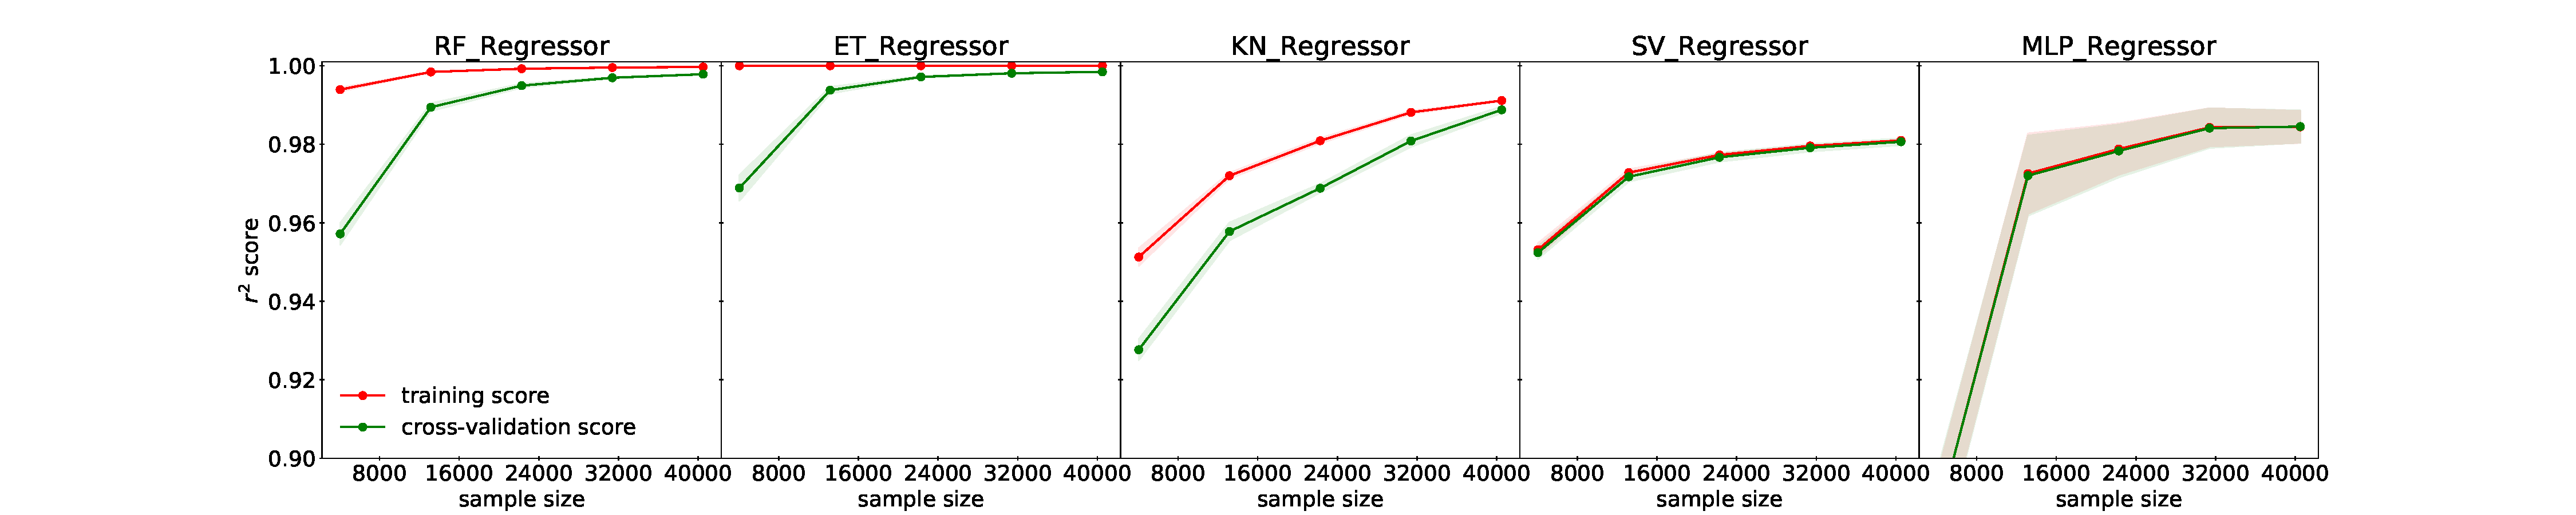
\includegraphics[trim=200 0 200 0, clip,
    		width=\textwidth]{images/regressors_learning_curves.pdf}

    		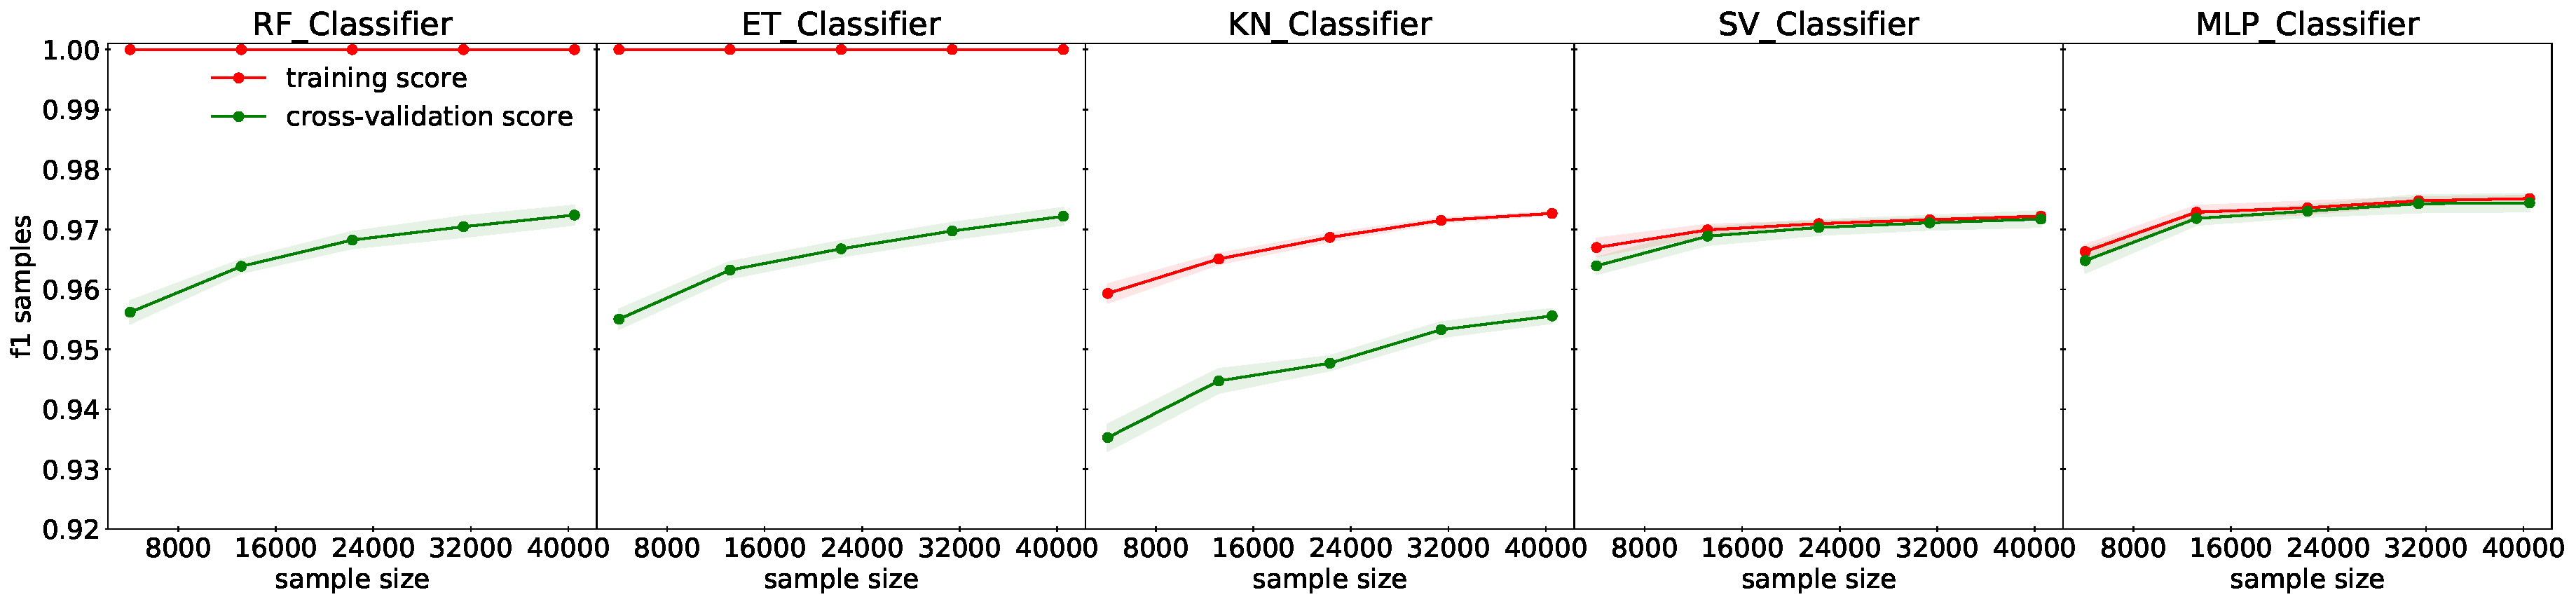
\includegraphics[width=\textwidth]{images/classifiers_learning_curves.pdf}
    	\end{center}
    	\caption{Learning curves of the selected estimators\DIFaddbeginFL \DIFaddFL{. Solid lines represent mean scores, while the shaded areas around lines represent the standard deviation of the mean due to error.}\DIFaddendFL }
    	\label{fig:lc}
    \end{figure}
%%%%%%%%%%%%%%%%%%%%%%%%%%%%%%%%%%%%%%%%
%%%%%%%%%%%%%%%%%%%%%%%%%%%%%%%%%%%%%%%%
\begin{table}[ht!]
	\centering
	\caption{Optimal \DIFdelbeginFL \DIFdelFL{hyper-parameters }\DIFdelendFL \DIFaddbeginFL \DIFaddFL{hyperparameters }\DIFaddendFL of the selected estimators}
	\DIFdelbeginFL %DIFDELCMD < \begin{tabular}{ll}
%DIFDELCMD < 		%%%
\DIFdelendFL \DIFaddbeginFL \begin{tabular}{l p{0.8\linewidth}}
%		\DIFaddendFL \hline
		\textbf{Method} & \textbf{Parameters  (Regressor/Classifier)} \\
        \hline
		\gls{RF} & \DIFdelbeginFL \DIFdelFL{max$\_$}\DIFdelendFL \DIFaddbeginFL \DIFaddFL{maximum }\DIFaddendFL features: None/None, \DIFdelbeginFL \DIFdelFL{n$\_$estimators}\DIFdelendFL \DIFaddbeginFL \DIFaddFL{number of trees}\DIFaddendFL : 400/400, \DIFdelbeginFL %DIFDELCMD < \\
%DIFDELCMD < 		                & %%%
\DIFdelFL{min$\_$samples$\_$leaf}\DIFdelendFL \DIFaddbeginFL \DIFaddFL{minimum number of samples}\DIFaddendFL : 7/7                 \\
		\gls{ET} & \DIFdelbeginFL \DIFdelFL{max$\_$}\DIFdelendFL \DIFaddbeginFL \DIFaddFL{maximum }\DIFaddendFL features: None/None, \DIFdelbeginFL \DIFdelFL{n$\_$estimators}\DIFdelendFL \DIFaddbeginFL \DIFaddFL{number of trees}\DIFaddendFL : 800/800, \DIFdelbeginFL %DIFDELCMD < \\
%DIFDELCMD < 		                & %%%
\DIFdelFL{min$\_$samples$\_$leaf}\DIFdelendFL \DIFaddbeginFL \DIFaddFL{minimum number of samples}\DIFaddendFL : 1/7, \DIFaddbeginFL \DIFaddFL{quality }\DIFaddendFL criterion: -/gini    \\
		\gls{KN} & \DIFdelbeginFL \DIFdelFL{weights}\DIFdelendFL \DIFaddbeginFL \DIFaddFL{weight function}\DIFaddendFL : distance/distance, \DIFdelbeginFL \DIFdelFL{n$\_$}\DIFdelendFL \DIFaddbeginFL \DIFaddFL{number of }\DIFaddendFL neighbors: 7/44, \DIFdelbeginFL %DIFDELCMD < \\
%DIFDELCMD < 		                & %%%
\DIFdelendFL \DIFaddbeginFL \DIFaddFL{distance }\DIFaddendFL metric: manhattan/manhattan, leaf \DIFdelbeginFL \DIFdelFL{$\_$}\DIFdelendFL size: 136/200  \\
		\DIFdelbeginFL %DIFDELCMD < \gls{SV}        %%%
\DIFdelendFL \DIFaddbeginFL \gls{SVM} \DIFaddendFL & kernel \DIFaddbeginFL \DIFaddFL{type}\DIFaddendFL : rbf/poly, \DIFaddbeginFL \DIFaddFL{polynomial }\DIFaddendFL degree: -/3, \DIFdelbeginFL \DIFdelFL{gamma}\DIFdelendFL \DIFaddbeginFL \DIFaddFL{kernel coefficient}\DIFaddendFL : auto/scale, \DIFdelbeginFL %DIFDELCMD < \\
%DIFDELCMD < 		                & %%%
\DIFdelendFL epsilon: 0.1/-, \DIFdelbeginFL \DIFdelFL{C}\DIFdelendFL \DIFaddbeginFL \DIFaddFL{regularization parameter}\DIFaddendFL : 3.4/1.2, \DIFdelbeginFL \DIFdelFL{tol}\DIFdelendFL \DIFaddbeginFL \DIFaddFL{stopping criterion}\DIFaddendFL : 1e-5 \\
		\gls{MLP} & activation \DIFaddbeginFL \DIFaddFL{function}\DIFaddendFL : relu/tanh, hidden \DIFdelbeginFL \DIFdelFL{$\_$layer$\_$sizes}\DIFdelendFL \DIFaddbeginFL \DIFaddFL{layers}\DIFaddendFL : 1000/250, \DIFdelbeginFL %DIFDELCMD < \\
%DIFDELCMD < 		                & %%%
\DIFdelFL{max$\_$iter}\DIFdelendFL \DIFaddbeginFL \DIFaddFL{maximum iterations}\DIFaddendFL : 1e4/1e4, tol: 1e-5, solver: adam/sgd, \DIFdelbeginFL %DIFDELCMD < \\
%DIFDELCMD < 		                & %%%
\DIFdelFL{learning $\_$}\DIFdelendFL \DIFaddbeginFL \DIFaddFL{learning }\DIFaddendFL rate: adaptive/constant       \\ \hline
	\end{tabular}
	\label{table:hyper}
\end{table}

\subsection{Final Estimators}
\DIFaddbegin

    \DIFaddend After performing the \DIFdelbegin \DIFdel{hyper-parameter }\DIFdelend \DIFaddbegin \DIFadd{hyperparameter }\DIFaddend optimization and learning curve \DIFdelbegin \DIFdel{assessments, we calculated }\DIFdelend \DIFaddbegin \DIFadd{assessment, we evaluated }\DIFaddend the final scores of the selected estimators and listed them in Table~\ref{table:finalreg} and ~\ref{table:finalclf}. At a \DIFdelbegin \DIFdel{quick
glance, }\DIFdelend \DIFaddbegin \DIFadd{glance, we saw that }\DIFaddend there is a slight enhancement in the performance scores of all regressors\DIFaddbegin \DIFadd{, }\DIFaddend except for the scores of \DIFaddbegin \DIFadd{the }\DIFaddend \gls{MLP} \DIFdelbegin \DIFdel{explicitly exhibiting a strong hyper-parameter dependency. On the other hand, optimization failed to improve classifier performance}\DIFdelend \DIFaddbegin \DIFadd{regressor that exhibits a strong hyperparameter dependency. However, the hyperparameter optimization did not improve the scores of the classifiers}\DIFaddend . With the optimized \DIFdelbegin \DIFdel{hyper-parameters and sample size in training}\DIFdelend \DIFaddbegin \DIFadd{hyperparameters and data size in the training dataset}\DIFaddend , the \gls{ET}, \DIFdelbegin %DIFDELCMD < \gls{SV}%%%
\DIFdelend \DIFaddbegin \gls{SVM}\DIFaddend , and \gls{MLP} regressors \DIFdelbegin \DIFdel{now predict
}\DIFdelend \DIFaddbegin \DIFadd{predicted }\DIFaddend performance metrics with a higher \DIFdelbegin \DIFdel{R$^2$ and lower mean absolute error (MAE)
compared to the }\DIFdelend \DIFaddbegin \gls{R2} \DIFadd{and lower }\gls{MAE} \DIFadd{compared to their }\DIFaddend preselection scores.

    \DIFdelbegin \DIFdel{Likewise, the }%DIFDELCMD < \gls{SV}  %%%
\DIFdelend \DIFaddbegin \DIFadd{On the other hand, the }\gls{SVM} \DIFaddend and \gls{MLP} classifiers \DIFdelbegin \DIFdel{label }\DIFdelend \DIFaddbegin \DIFadd{labeled }\DIFaddend the design attributes \DIFdelbegin \DIFdel{,
providing a higher average precision (AP) and lower label ranking loss (LRL).
The }%DIFDELCMD < \gls{MLP} %%%
\DIFdel{and }%DIFDELCMD < \gls{ET} %%%
\DIFdel{methods demonstrate the lowest errors }\DIFdelend \DIFaddbegin \DIFadd{with the highest }\gls{AP} \DIFadd{and lowest }\gls{LRL} \DIFadd{scores }\DIFaddend relative to the other estimators\DIFdelbegin \DIFdel{and one accordingly promising candidates for the subsequent
phase of this study. To select the right estimator(s) }\DIFdelend \DIFaddbegin \DIFadd{. Nonetheless, the others are also suitable as all the scores are very close to each other. As the scores did not give us sufficient information about determining the right estimator }\DIFaddend for the next phase, \DIFdelbegin \DIFdel{the
}\DIFdelend \DIFaddbegin \DIFadd{we investigated }\DIFaddend cross-validation plots and multi-label confusion matrices \DIFaddbegin \DIFadd{on the basis }\DIFaddend of each performance metric (i.e., $k_{\infty}$, $\varsigma$, $\phi_{fast}$)\DIFdelbegin \DIFdel{must be investigated}\DIFdelend .

%%%%%%%%%%%%%%%%%%%%%%%%%%%%%%%%%%%%%%%%
    \begin{table}[ht!]
    	\centering
    	\caption{\DIFdelbeginFL \DIFdelFL{Performance }\DIFdelendFL \DIFaddbeginFL \DIFaddFL{Final performance }\DIFaddendFL scores \DIFdelbeginFL \DIFdelFL{for }\DIFdelendFL \DIFaddbeginFL \DIFaddFL{of }\DIFaddendFL the selected regressors}
    	\begin{tabular}{lllll>{\columncolor[gray]{0.9}}l}
    		\hline
    		& \textbf{\gls{RF}}  & \textbf{\gls{ET}}  & \textbf{\gls{KN}} &
    		\textbf{\DIFdelbeginFL %DIFDELCMD < \gls{SV}%%%
\DIFdelendFL \DIFaddbeginFL \gls{SVM}\DIFaddendFL }   & \textbf{\gls{MLP}} \\
    		\hline
    		\DIFdelbeginFL \DIFdelFL{$fit$\_$score$  }\DIFdelendFL \DIFaddbeginFL \DIFaddFL{fit score  }\DIFaddendFL & 1.00 	& 1.00 & 1.00 & 0.97  & 1.00 \\
    		\DIFdelbeginFL \DIFdelFL{EVR }\DIFdelendFL \DIFaddbeginFL \gls{EVR} \DIFaddendFL & 0.94 & 0.99 & 0.99 & 0.96 & 1.00 \\
    		\gls{MAE} & 1.07 & 0.28 & 0.41 & 0.37 & 0.23 \\
    		\gls{MSE} & 5.52 & 0.41 & 0.83 & 0.44 & 0.24 \\
    		R$^2$ & 0.94 & 0.99 & 0.98 & 0.96 & 1.00 \\
    		\hline
    	\end{tabular}
    	\label{table:finalreg}
    \end{table}
%%%%%%%%%%%%%%%%%%%%%%%%%%%%%%%%%%%%%%%%
    \begin{table}[ht!]
    	\centering
    	\caption{\DIFdelbeginFL \DIFdelFL{Performance }\DIFdelendFL \DIFaddbeginFL \DIFaddFL{Final performance }\DIFaddendFL scores \DIFdelbeginFL \DIFdelFL{for }\DIFdelendFL \DIFaddbeginFL \DIFaddFL{of }\DIFaddendFL the selected classifiers}
    	\begin{tabular}{lllll>{\columncolor[gray]{0.9}}l}
    		\hline
    		& \textbf{\gls{RF}} & \textbf{\gls{ET}}  & \textbf{\gls{KN}} &
    		\textbf{\DIFdelbeginFL %DIFDELCMD < \gls{SV}%%%
\DIFdelendFL \DIFaddbeginFL \gls{SVM}\DIFaddendFL }  & \textbf{\gls{MLP}} \\
    		\hline
    		\DIFdelbeginFL \DIFdelFL{$fit$\_$score$  }\DIFdelendFL \DIFaddbeginFL \DIFaddFL{fit score  }\DIFaddendFL & 0.93 & 1.00 & 1.00  & 0.89 & 0.90 \\
    		\DIFdelbeginFL \DIFdelFL{AP }\DIFdelendFL \DIFaddbeginFL \gls{AP} \DIFaddendFL & 0.92 & 0.94 & 0.95  & 0.96 & 0.97  \\
    		\gls{HL} & 0.04 & 0.04 & 0.04  & 0.03 & 0.03  \\
    		\DIFdelbeginFL \DIFdelFL{LRAPS  }\DIFdelendFL \DIFaddbeginFL \gls{LRAPS}  \DIFaddendFL & 0.95 & 0.96 & 0.96  & 0.96 & 0.97 \\
    		\gls{LRL} & 0.07 & 0.06 & 0.06  & 0.05 & 0.05  \\
    		\DIFdelbeginFL \DIFdelFL{ROCAUC }\DIFdelendFL \DIFaddbeginFL \gls{ROCAUC} \DIFaddendFL & 0.94 & 0.95 & 0.96  & 0.95 & 0.96 \\
    		\hline
    	\end{tabular}
    	\label{table:finalclf}
    \end{table}
%%%%%%%%%%%%%%%%%%%%%%%%%%%%%%%%%%%%%%%%

\subsection{Cross-validation \DIFaddbegin \DIFadd{plot }\DIFaddend and confusion matrix}
\DIFaddbegin

    \DIFadd{In this section, we compared the predicted test dataset with the actual test dataset. }\DIFaddend Figure~\ref{fig:cv} visualizes the predicted performance \DIFdelbegin \DIFdel{metric values }\DIFdelend \DIFaddbegin \DIFadd{metrics }\DIFaddend against their actual values for \DIFdelbegin \DIFdel{each estimator. The }\DIFdelend \DIFaddbegin \DIFadd{the chosen estimators in terms of }\DIFaddend cross-validation plots\DIFdelbegin \DIFdel{reveal how an
estimatoracts on an individual basis of performance metrics within the 5\%
relative error region and show only three (}\DIFdelend \DIFaddbegin \DIFadd{. These plots show the estimator's prediction quality separately for each performance metric. Results indicated that the }\DIFaddend \gls{ET}, \gls{KN}, and \gls{MLP} \DIFdelbegin \DIFdel{) of
the }\DIFdelend estimators accurately predict \DIFdelbegin \DIFdel{the performance metrics in accordance with }\DIFdelend \DIFaddbegin \DIFadd{performance metrics per }\DIFaddend the acceptance criterion \DIFaddbegin \DIFadd{(within $<$5\% relative error)}\DIFaddend .

    \DIFdelbegin \DIFdel{With the given training sample size and hyper-parameters}\DIFdelend \DIFaddbegin \DIFadd{According to these results}\DIFaddend , the \gls{ET} \DIFaddbegin \DIFadd{estimator }\DIFaddend is the best option to \DIFdelbegin \DIFdel{be used }\DIFdelend \DIFaddbegin \DIFadd{employ }\DIFaddend in the optimization phase. \DIFdelbegin \DIFdel{With respect to }\DIFdelend \DIFaddbegin \DIFadd{In comparison to the }\DIFaddend actual values, it correctly estimated \DIFaddbegin \DIFadd{the }\DIFaddend $k_{\infty}$ \DIFaddbegin \DIFadd{metric}\DIFaddend , slightly underestimated \DIFaddbegin \DIFadd{the }\DIFaddend $\varsigma$ \DIFaddbegin \DIFadd{metric}\DIFaddend , and predicted a few values of the $\phi_{fast}$ metric outside of the region. The \gls{KN} and \gls{MLP} \DIFdelbegin \DIFdel{have }\DIFdelend \DIFaddbegin \DIFadd{estimators have good }\DIFaddend results comparable to the \gls{ET} and\DIFdelbegin \DIFdel{may therefore}\DIFdelend \DIFaddbegin \DIFadd{, therefore, }\DIFaddend be considered as alternative estimators for \DIFdelbegin \DIFdel{the regression analysisof channel
designs}\DIFdelend \DIFaddbegin \DIFadd{regression analysis}\DIFaddend .

    For classification analysis, we presented \DIFdelbegin \DIFdel{the }\DIFdelend confusion matrices, normalized over the total test sample size, in Figure~\ref{fig:cm} to compare the predicted labels with the actual labels \DIFdelbegin \DIFdel{by defining the responses }\DIFdelend in terms of true/false positive and true/false negative scores. From the prediction capability standpoint, these estimators have very close scores in each label and predict all labels with \DIFdelbegin \DIFdel{a high precision of more than }\DIFdelend \DIFaddbegin \DIFadd{high precision ($<$}\DIFaddend 95\%\DIFaddbegin \DIFadd{)}\DIFaddend . Related to the scores of the labels, the only label that causes the highest misclassification score by 10\% is the feedback coefficient. This mislabeling originates from the feedback coefficients very close to zero \DIFdelbegin \DIFdel{, which may not be accurately estimatedas they
inevitably carry a prediction error. The other labels are }\DIFdelend \DIFaddbegin \DIFadd{as they are not accurately estimated. Other labels were, however, }\DIFaddend correctly estimated with an error of less than 1\%. As a result, \DIFdelbegin \DIFdel{one }\DIFdelend \DIFaddbegin \DIFadd{any }\DIFaddend of these classifiers can easily handle the classification of channel designs without \DIFaddbegin \DIFadd{causing a }\DIFaddend notable loss in labeling. In this context, as in the regression analysis, we decided to use the \gls{ET} classifier in the design optimization phase \DIFdelbegin \DIFdel{of this study to assess the dedicated }\DIFdelend \DIFaddbegin \DIFadd{to estimate the }\DIFaddend labels of optimum designs.

    \begin{figure}[ht!]
     \begin{center}
            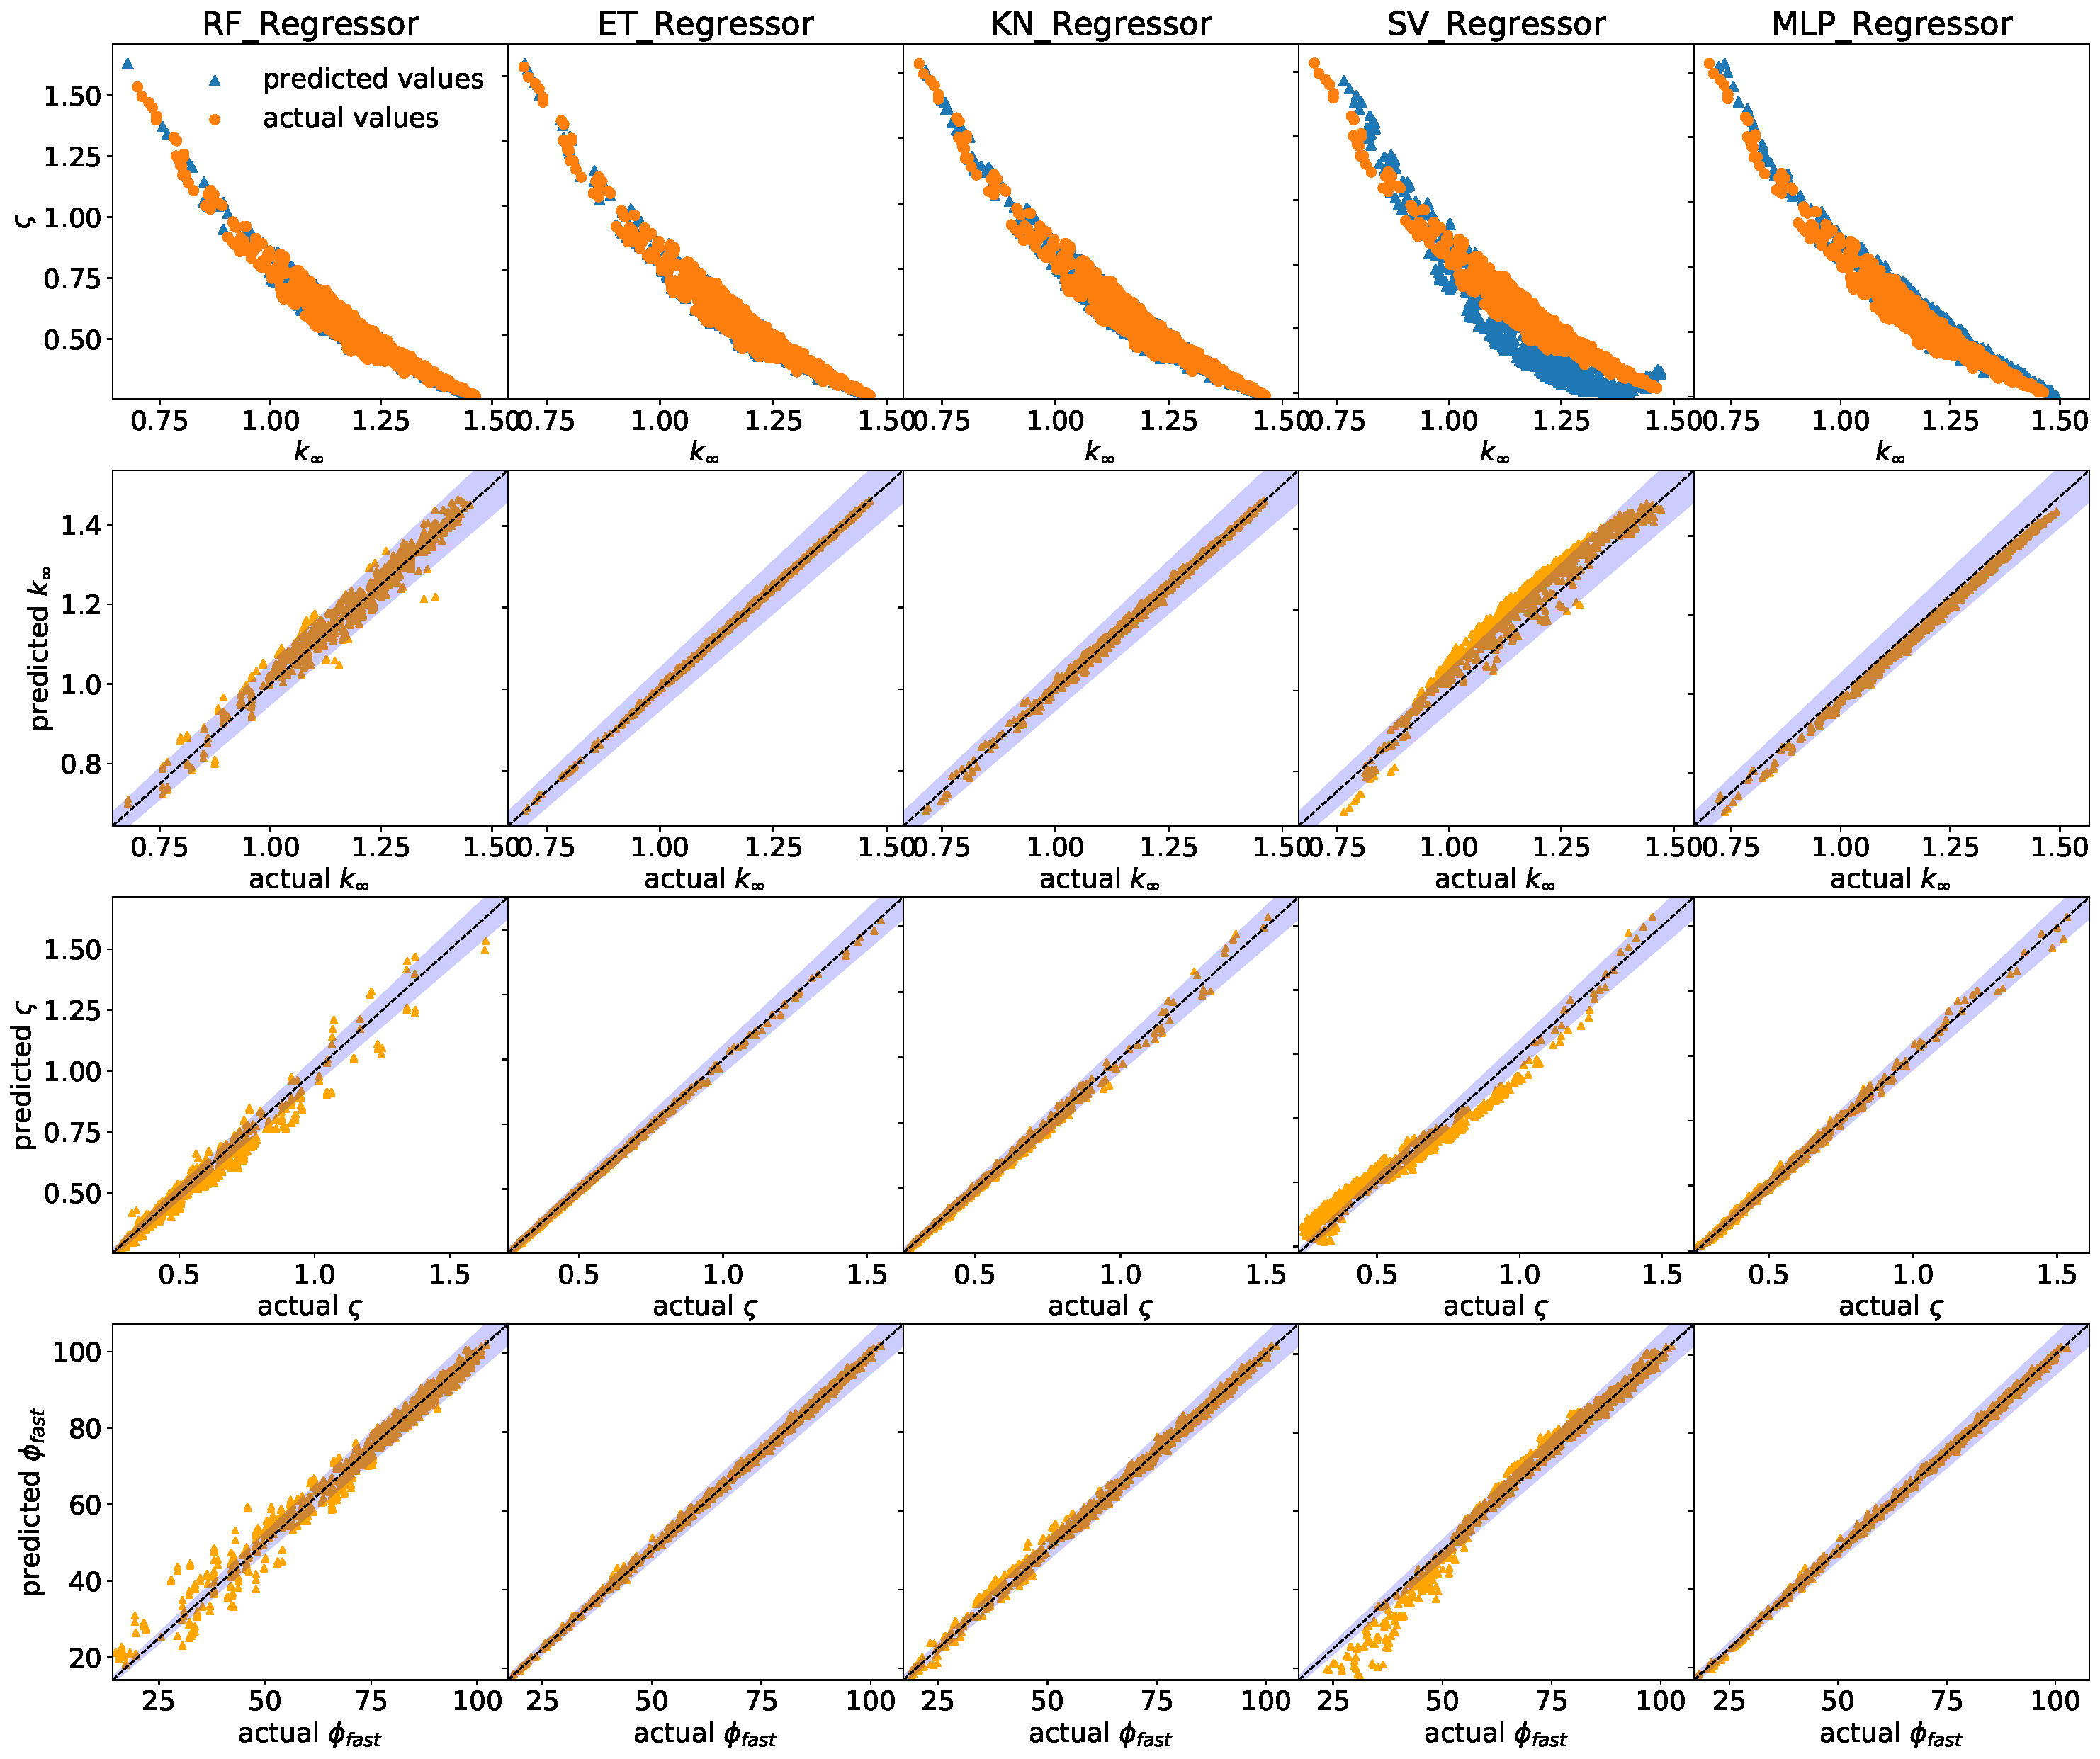
\includegraphics[width=\textwidth]{images/regression_cross_validation.pdf}
     \end{center}
        \caption{Cross-validation plots of the selected regressors, top to bottom:	(i)$k_{\infty}$ versus $\varsigma$ (ii) $k_{\infty}$ (iii) $\varsigma$ and	(iv) $\phi_{fast}$  }
        \label{fig:cv}
    \end{figure}
    \begin{figure}[htbp!]
     \begin{center}
            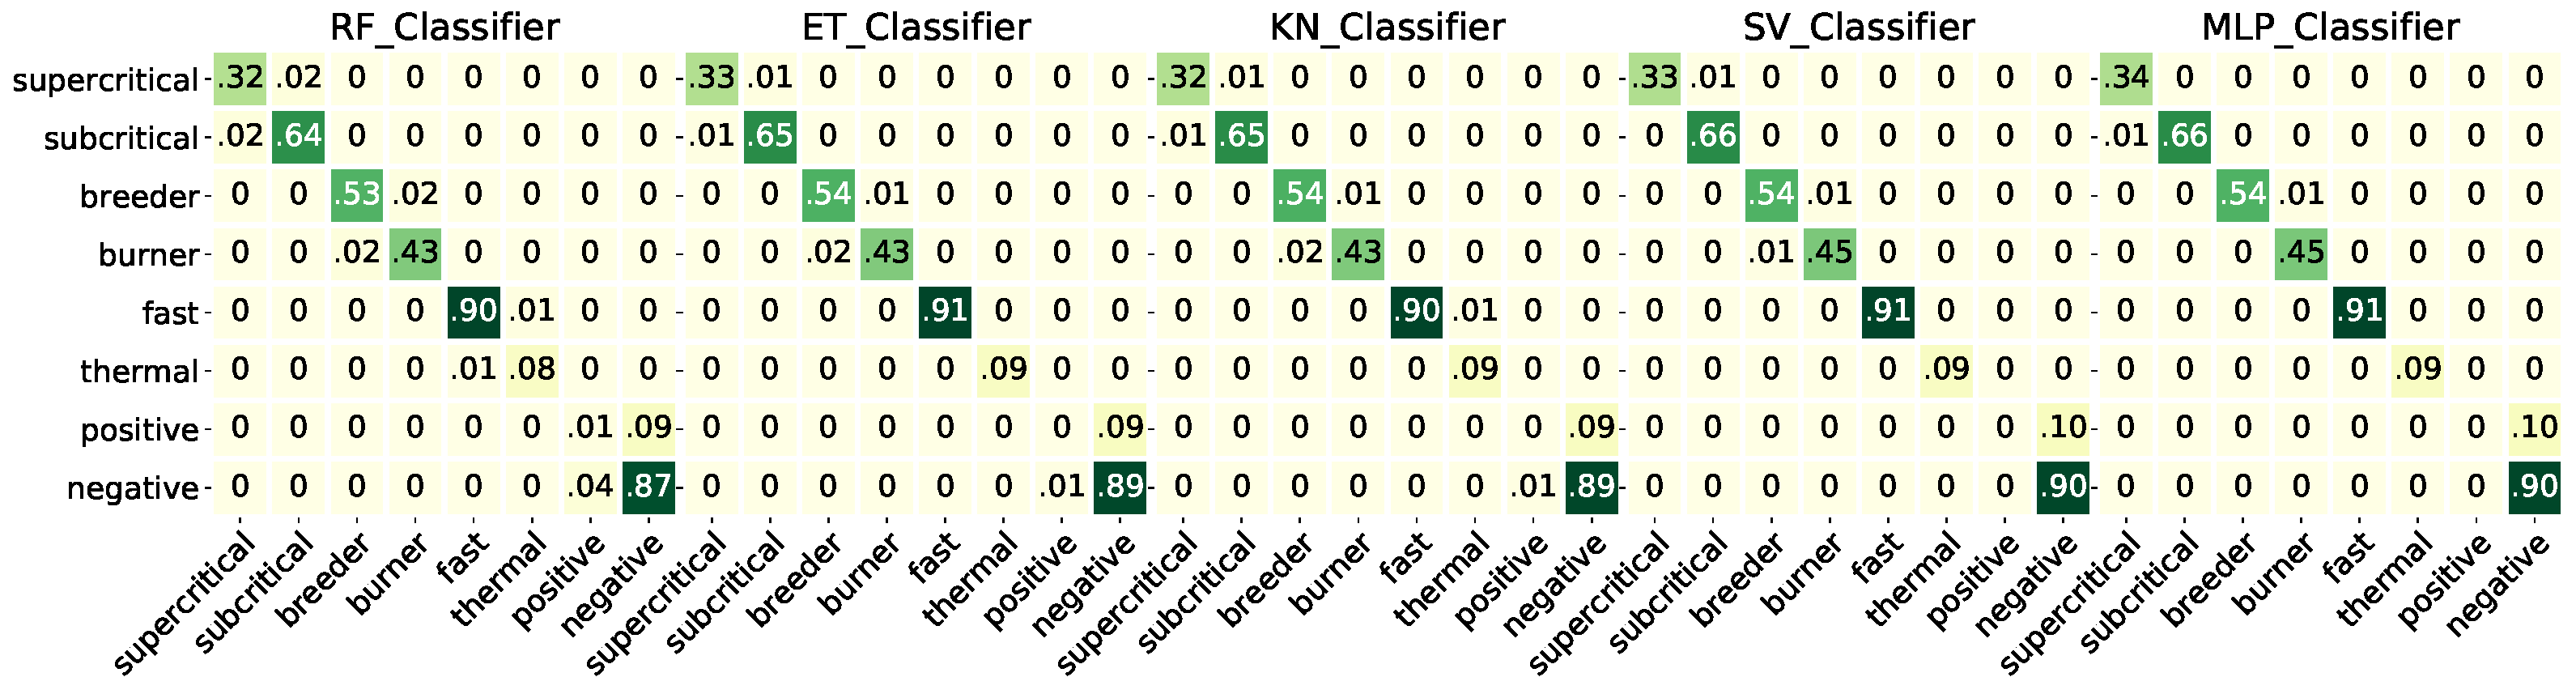
\includegraphics[width=\textwidth]{images/classification_confusion_matrix.pdf}
     \end{center}
        \caption{Normalized confusion matrices of the selected classifiers}
        \label{fig:cm}
    \end{figure}

\subsection{Optimum Designs}
\DIFdelbegin \DIFdel{In accordance with }\DIFdelend \DIFaddbegin

    \DIFadd{Based on }\DIFaddend the constraints applied to \DIFdelbegin \DIFdel{the }\DIFdelend performance metrics, we found a set of optimum solutions for each fuel-salt pair. As an illustration, \DIFdelbegin \DIFdel{Figure~\ref{fig:pareto} depicts the pareto-front }\DIFdelend \DIFaddbegin \DIFadd{we presented the Pareto-front }\DIFaddend solutions for the (U-Th)F$_4$-NaF-BeF$_2$, \DIFaddbegin \DIFadd{which is very }\DIFaddend similar to the results of other fuel-salt pairs\DIFdelbegin \DIFdel{. The
}\DIFdelend \DIFaddbegin \DIFadd{, in Figure~\ref{fig:pareto}. This }\DIFaddend figure includes (a) \DIFdelbegin \DIFdel{the }\DIFdelend cross-validation plots for each performance metric, (b) the distribution of the \DIFdelbegin \DIFdel{pareto-front }\DIFdelend \DIFaddbegin \DIFadd{Pareto-front }\DIFaddend solutions in 3-D performance metric space, and (c) the normalized confusion matrix\DIFdelbegin \DIFdel{for the classification results. From }\DIFdelend \DIFaddbegin \DIFadd{. As seen from }\DIFaddend the subplot (a), the \DIFdelbegin \DIFdel{pareto-optimal }\DIFdelend \DIFaddbegin \DIFadd{Pareto-optimal }\DIFaddend solutions (blue triangle) \DIFdelbegin \DIFdel{overlap }\DIFdelend \DIFaddbegin \DIFadd{overlapped }\DIFaddend very well with the actual values (orange circles)\DIFdelbegin \DIFdel{obtained by the Serpent simulation. Additionally, the solutions show convex distribution in agreement with the
distribution shown in the uppermost subplot of Figure ~\ref{fig:cv}. This
situation can be easily observed from the subplot (b). }\DIFdelend \DIFaddbegin \DIFadd{. }\DIFaddend The other subplots also confirm this situation by showing good distributions in the very proximity of the intersection line of each performance metric.

    The cross-validation subplots also \DIFdelbegin \DIFdel{indicate that }\DIFdelend \DIFaddbegin \DIFadd{indicated that all }\DIFaddend the predicted metrics totally stay within \DIFaddbegin \DIFadd{the }\DIFaddend 5\% relative error (\DIFdelbegin \DIFdel{shaded-area) }\DIFdelend \DIFaddbegin \DIFadd{shaded area) and }\DIFaddend very close to the intersection line. We found even better results for the $k_{\infty}$ \DIFaddbegin \DIFadd{metric }\DIFaddend with no more than 1\% relative error.

    \DIFdelbegin \DIFdel{Like the validation of the solutions obtained by the regression analysis }\DIFdelend \DIFaddbegin \DIFadd{As in the regression analysis results}\DIFaddend , the classification results of the optimal solutions in subplot (c) \DIFdelbegin \DIFdel{, agree }\DIFdelend \DIFaddbegin \DIFadd{agreed }\DIFaddend very well with the actual labels. The only noteworthy complication is the misclassification of a tiny fraction of the feedback indicators. This mislabeling certainly \DIFdelbegin \DIFdel{arises }\DIFdelend \DIFaddbegin \DIFadd{arose }\DIFaddend from the prediction of the ${\alpha_{total}}$ values \DIFaddbegin \DIFadd{as }\DIFaddend discussed before and \DIFdelbegin \DIFdel{are }\DIFdelend \DIFaddbegin \DIFadd{were }\DIFaddend estimated as positive instead of negative. In conformity with the constraints applied to \DIFdelbegin \DIFdel{the }\DIFdelend performance metrics in the optimization phase, all the optimum designs we found are of characteristics of supercritical eigenvalue, fast spectrum, burner type\DIFaddbegin \DIFadd{, }\DIFaddend and negative feedback.

    Of the entire Pareto front solutions (around 650) \DIFdelbegin \DIFdel{accounting }\DIFdelend \DIFaddbegin \DIFadd{which account }\DIFaddend for each combination of the fuel-salt pairs, only the nine best solutions are tabulated in Table~\ref{table:optimaldesigns}. We simply opted for the solutions that grant the highest breeding ratio ($\varsigma$) and the lowest fast flux ($\phi_{fast}$) at the $k_{\infty}$ = 1.06. The only exception for the multiplication factor criterion is for the NaCl salt in U-Pu fuel as \DIFdelbegin \DIFdel{no
}\DIFdelend \DIFaddbegin \DIFadd{there are no solutions with a }\DIFaddend multiplication factor less than 1.21 \DIFdelbegin \DIFdel{has been found }\DIFdelend for this fuel-salt pair.

    \DIFdelbegin \DIFdel{From }\DIFdelend \DIFaddbegin \DIFadd{As provided in }\DIFaddend the table, the suggested solutions can be grouped more easily by fuel type \DIFdelbegin \DIFdel{,
as provided in the table, as the }\DIFdelend \DIFaddbegin \DIFadd{as the }\DIFaddend solutions show a certain relationship with the fuel type rather than \DIFaddbegin \DIFadd{the }\DIFaddend salt type. When \DIFdelbegin \DIFdel{different }\DIFdelend \DIFaddbegin \DIFadd{the }\DIFaddend fuel types are compared to each other, \DIFdelbegin \DIFdel{the }\DIFdelend U-Th \DIFdelbegin \DIFdel{fuel requires }\DIFdelend \DIFaddbegin \DIFadd{fuels require }\DIFaddend the highest $^{235}$U content (18-20\%) due to the existence of the $^{232}$Th isotope which has an absorption cross-section approximately four times higher than $^{238}$U. U \DIFdelbegin \DIFdel{fuel reaches its }\DIFdelend \DIFaddbegin \DIFadd{fuels reach their }\DIFaddend top performance when a moderate amount of $^{235}$U (14-15\%) is used. U-Pu \DIFdelbegin \DIFdel{fuel
needs }\DIFdelend \DIFaddbegin \DIFadd{fuels need }\DIFaddend the lowest amount of $^{235}$U (5\%) as not only does Pu in U-Pu already contain a certain fraction of fissile isotopes like $^{239}$Pu and $^{241}$Pu, but also Pu fissile isotopes emit greater average fission neutrons per absorption. \DIFdelbegin \DIFdel{In a similar way}\DIFdelend \DIFaddbegin \DIFadd{Similarly}\DIFaddend , we noticed that \DIFdelbegin \DIFdel{the }\DIFdelend U-Th \DIFdelbegin \DIFdel{fuel demands about
}\DIFdelend \DIFaddbegin \DIFadd{fuels demand }\DIFaddend 13-14\% Th in U-Th while \DIFdelbegin \DIFdel{the }\DIFdelend U-Pu \DIFdelbegin \DIFdel{fuel favors }\DIFdelend \DIFaddbegin \DIFadd{fuels favor }\DIFaddend the highest grade of U content (90\%).

    A comprehensive look at the common properties of the optimal designs suggests that $T_{ave}$ should be in the range of 1100-1200 K and $\xi$ needs to be at its minimum value \DIFdelbegin \DIFdel{of }\DIFdelend \DIFaddbegin \DIFadd{(}\DIFaddend 0.274\DIFaddbegin \DIFadd{)}\DIFaddend . Furthermore, as expected, Th necessitates higher fissile material than any other fuel \DIFdelbegin \DIFdel{type }\DIFdelend \DIFaddbegin \DIFadd{types }\DIFaddend whereas the fissile material required by the U-Pu fuel is the lowest as the \DIFdelbegin \DIFdel{Pu coming from the }\DIFdelend weapons-grade \DIFdelbegin \DIFdel{already
comprises a great }\DIFdelend \DIFaddbegin \DIFadd{Pu comprises a gread }\DIFaddend deal of fissile isotopes by almost 50\% of its content. On the other hand, unlike \DIFaddbegin \DIFadd{the }\DIFaddend other feature parameters \DIFdelbegin \DIFdel{displaying }\DIFdelend \DIFaddbegin \DIFadd{that display }\DIFaddend a direct characteristic relationship with the fuel type, there is no noticeable evidence to associate the channel-to-channel pitch length ($p$) with the fuel types\DIFdelbegin \DIFdel{but the }\DIFdelend \DIFaddbegin \DIFadd{. The }\DIFaddend $p$ \DIFdelbegin \DIFdel{is
}\DIFdelend \DIFaddbegin \DIFadd{parameter is, however, }\DIFaddend likely to vary with the salt type \DIFdelbegin \DIFdel{. As an example, the NaCl }\DIFdelend \DIFaddbegin \DIFadd{just as the NaCl salt }\DIFaddend calls for a constant pitch value of 1.0 cm in all fuel types.

    \DIFdelbegin \DIFdel{Overall}\DIFdelend \DIFaddbegin \DIFadd{In summary}\DIFaddend , among the \DIFaddbegin \DIFadd{optimal }\DIFaddend designs, it appears that all the fuels mixed with the NaCl salt are the most promising designs. In particular, the \DIFdelbegin \DIFdel{UF}\DIFdelend \DIFaddbegin \DIFadd{F}\DIFaddend $_4$-PuF$_3$-NaCl fuel-salt yields the highest $\varsigma$ and $k_{\infty}$. The most unfavorable side of this fuel-salt is to have a lower ${\alpha_{total}}$ than other salt types but the coefficient is still quite sufficient compared to the \DIFdelbegin \DIFdel{current
}\DIFdelend \DIFaddbegin \DIFadd{exiting }\DIFaddend designs of \gls{MSR}s at the initial state with a total \DIFdelbegin \DIFdel{fuel salt }\DIFdelend \DIFaddbegin \DIFadd{fuel-salt }\DIFaddend feedback coefficient of around -3.4 pcm/K \cite{rykhlevskii2019, robertson1971}. From the reactor safety point of view, \DIFdelbegin \DIFdel{with the highest ${\alpha_{total}}$, the
}\DIFdelend \DIFaddbegin \DIFadd{the }\DIFaddend LiF-BeF$_2$ salt \DIFaddbegin \DIFadd{with the highest ${\alpha_{total}}$ }\DIFaddend is the most favorable.

    \begin{figure*}
    	\begin{center}
    		\begin{minipage}{.49\linewidth}
    			\DIFdelbeginFL %DIFDELCMD < \begin{subfigure}[t]{0.8\linewidth}
%DIFDELCMD < 				%%%
\DIFdelendFL \DIFaddbeginFL \begin{subfigure}[t]{1.0\linewidth}
    				\DIFaddendFL 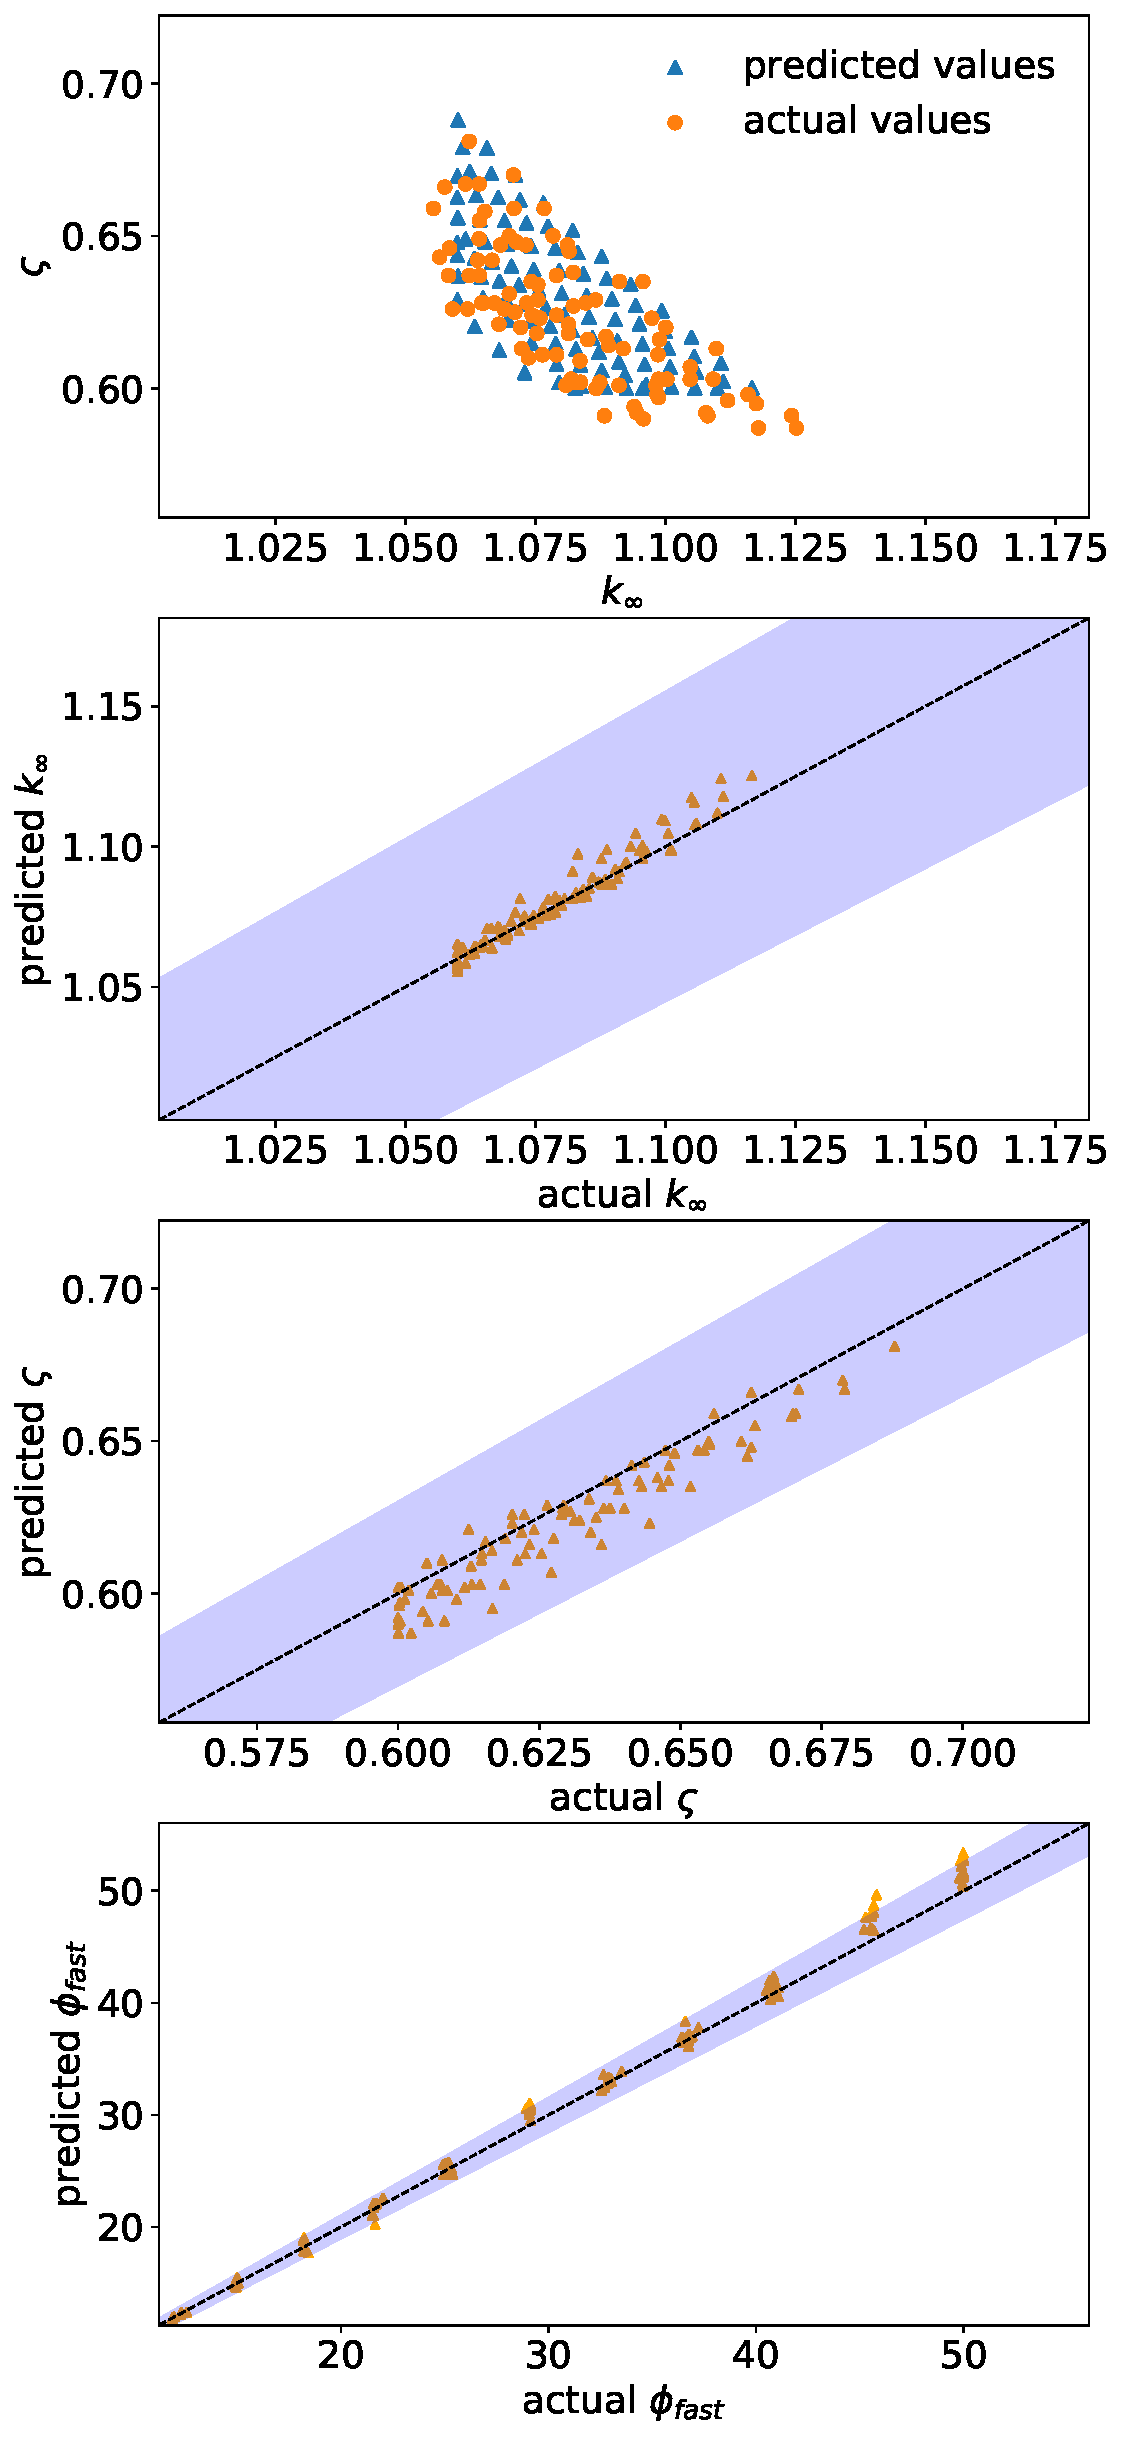
\includegraphics[width=\textwidth]{images/22_optimal_design_cross_validation.pdf}
    				\caption{}
    			\end{subfigure}
    		\end{minipage}
    		\begin{minipage}{.49\linewidth}
    			\DIFdelbeginFL %DIFDELCMD < \begin{subfigure}[t]{0.8\linewidth}
%DIFDELCMD < 				%%%
\DIFdelendFL \DIFaddbeginFL \begin{subfigure}[t]{1.0\linewidth}
    				\DIFaddendFL 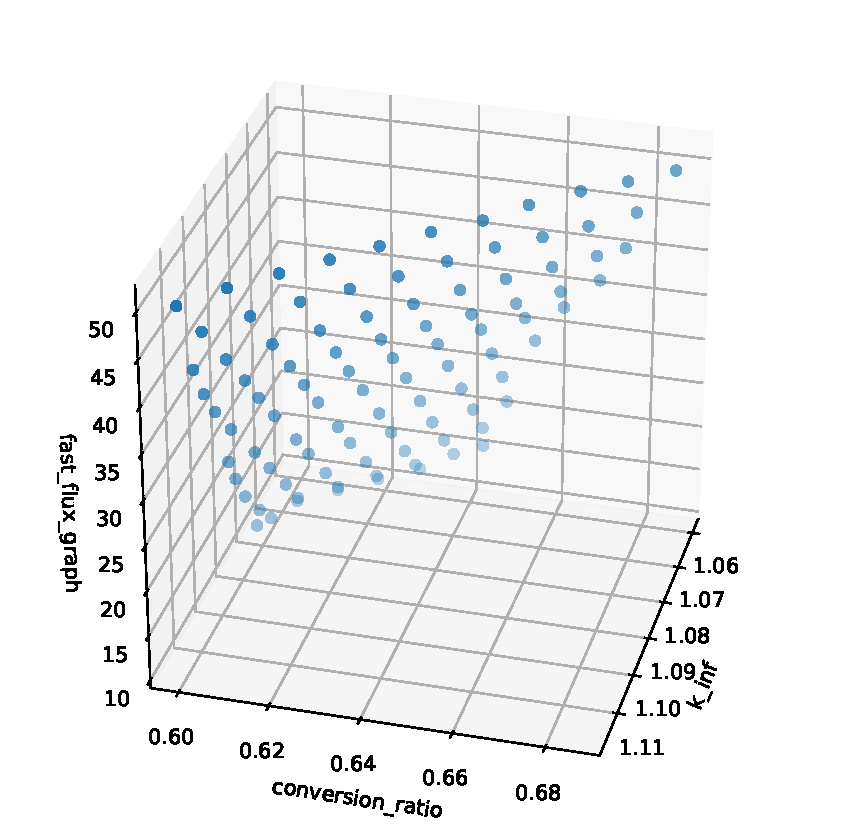
\includegraphics[width=\textwidth]{images/22_optimal_design_3d_solutions.pdf}
    				\caption{}
    			\end{subfigure} \\
    			\DIFdelbeginFL %DIFDELCMD < \begin{subfigure}[b]{0.8\linewidth}
%DIFDELCMD < 				%%%
\DIFdelendFL \DIFaddbeginFL \begin{subfigure}[b]{1.0\linewidth}
    				\DIFaddendFL 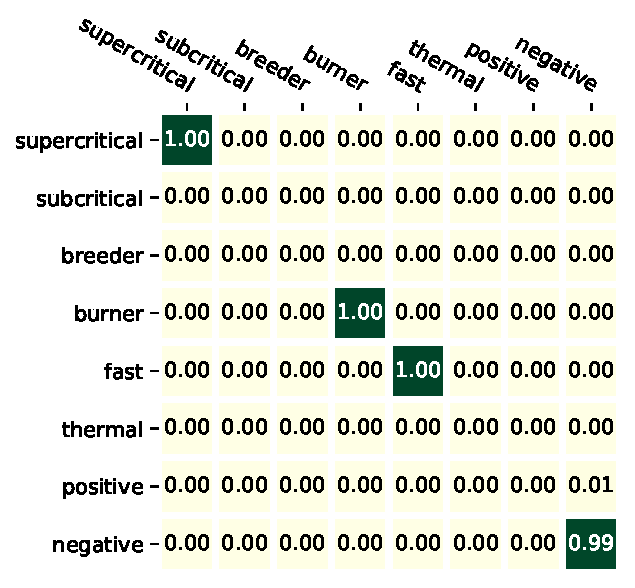
\includegraphics[width=\textwidth]{images/22_optimal_design_confusion_matrix.pdf}
    				\caption{}
    			\end{subfigure}
    		\end{minipage}
    	\end{center}
    	\caption{Optimum solutions for (U-Th)F$_4$-NaF-BeF$_2$: (a) cross-validation plots of performance metrics, (b) \DIFaddbeginFL \DIFaddFL{the }\DIFaddendFL distribution of the \DIFdelbeginFL \DIFdelFL{pareto-front }\DIFdelendFL \DIFaddbeginFL \DIFaddFL{Pareto-front }\DIFaddendFL solutions in 3-D performance metric space, and (c) \DIFaddbeginFL \DIFaddFL{the }\DIFaddendFL normalized confusion matrix.}
    	\label{fig:pareto}
    \end{figure*}


%%%%%%%%%%%%%%%%%%%%%%%%%%%%%%%%%%%%%%%%
\begin{landscape}
	\begin{table}[ht!]
		\centering
		\caption{\DIFdelbeginFL \DIFdelFL{Selected best }\DIFdelendFL \DIFaddbeginFL \DIFaddFL{Optimal }\DIFaddendFL designs for each fuel-salt pair\DIFdelbeginFL %DIFDELCMD < \tnote{$\star$}%%%
\DIFdelendFL \DIFaddbeginFL \DIFaddFL{$^\star$}\DIFaddendFL }
		\begin{threeparttable}[t]
			\begin{tabular}{lllllllllll}
				\hline
				\textbf{Fuel Type} & \textbf{Salt Type}  & \textbf{$f_{35}$} &
				\textbf{$f_{U}$} & \textbf{$p$}	& \textbf{$T_{ave}$} & \textbf{$\xi$} &
				\textbf{$k_{\infty}$ \tnote{$\dagger$}}	& \textbf{$\varsigma$
					\tnote{$\ddagger$}}  & \textbf{$\phi_{fast}$ \tnote{$\perp$}} &
				\textbf{${\alpha_{total}}$ 	\tnote{$\wedge$}}  \\
				\hline

				U 	& LiF-BeF$_2$ 	& 14.47 & 100.0 & 86.7 & 1200 & 0.274 & 1.0600(+60) &
				0.661(-6) & 18.6(-0.5) 	& -3.9\\
				U 	& NaF-BeF$_2$ 	& 14.88 & 100.0 & 7.18 & 1125 & 0.274 & 1.0600(-120) &
				0.638(+6) & 19.0(-0.9) 	& -4.0\\
				U 	& NaCl 	& 14.28 & 100.0 & 1.00 & 1176 & 0.274 & 1.0604(-20) &
				0.692(0) & 12.6(0) 	& -3.0\\
				U-Th & LiF-BeF$_2$ 	& 19.10	& 86.7 & 5.50 & 1123 & 0.276 & 1.0601(-70) &
				0.665(-7) & 17.1(-0.2) 	& -4.3\\
				U-Th & NaF-BeF$_2$ 	& 20.00 & 86.8 & 5.98 & 1125 & 0.275 & 1.0600(+30) &
				0.643(-11) & 16.0(-0.2) & -2.8\\
				U-Th 	& NaCl 	& 18.48	& 86.2 	& 1.00 	& 1199 & 0.274 & 1.0600(+140) 	&
				0.696(-1) & 14.4(0)	& -2.8\\
				U-Pu & LiF-BeF$_2$ 	& 5.00 	& 90.0 	& 4.40 	& 1198 & 0.274 & 1.0600(-20) &
				0.732(+3) & 16.0(0.2) & -4.5\\
				U-Pu	& NaF-BeF$_2$ 	& 5.00 	& 89.3 & 4.37 & 1125 & 0.275 & 1.0600(+460) &
				0.723(+15) & 13.6(0.3) 	& -3.3\\
				U-Pu	& NaCl & 5.00 & 90.0 & 1.00 & 1193 	& 0.274 & 1.2192(+10) &
				0.753(+1) & 13.0(0)	& -3.4\\
				\hline
			\end{tabular}
            \DIFdelbeginFL %DIFDELCMD < \begin{tablenotes}
%DIFDELCMD < 				\item[$\star$] %%%
\DIFdelendFL \DIFaddbeginFL \DIFaddFL{\rule{0in}{1.2em}$^\star$}\scriptsize \DIFaddendFL Performance metrics given in the table are the predicted values. The \DIFdelbeginFL \DIFdelFL{actual values are given within the brackets }\DIFdelendFL \DIFaddbeginFL \DIFaddFL{values inside the brackets are the actual values }\DIFaddendFL in terms of \DIFdelbeginFL \DIFdelFL{differences
				}\DIFdelendFL \DIFaddbeginFL \DIFaddFL{difference }\DIFaddendFL from the predicted values.
\DIFdelbeginFL %DIFDELCMD < \item[$\dagger$] %%%
\DIFdelFL{Computational error of }\DIFdelendFL \DIFaddbeginFL

			\DIFaddFL{\rule{0in}{1.2em}$^\dagger$}\scriptsize \DIFaddFL{The computational error of the }\DIFaddendFL infinite multiplication factor is $\pm$0.0009. The values within the brackets are in the units of pcm.
\DIFdelbeginFL %DIFDELCMD < \item[$\ddagger$] %%%
\DIFdelFL{Computational error of }\DIFdelendFL \DIFaddbeginFL

			\DIFaddFL{\rule{0in}{1.2em}$^\ddagger$}\scriptsize \DIFaddFL{The computational error of the }\DIFaddendFL conversion ratio is $\pm$0.005. The values within the brackets are in the units of milli.
\DIFdelbeginFL %DIFDELCMD < \item[$\perp$] %%%
\DIFdelFL{Computational error of }\DIFdelendFL \DIFaddbeginFL

			\DIFaddFL{\rule{0in}{1.2em}$^\perp$}\scriptsize \DIFaddFL{The computational error of the }\DIFaddendFL fast flux is $\pm$0.007.
\DIFdelbeginFL %DIFDELCMD < \item[$\wedge$] %%%
\DIFdelFL{Propagated }\DIFdelendFL \DIFaddbeginFL

			\DIFaddFL{\rule{0in}{1.2em}$^\wedge$}\scriptsize \DIFaddFL{The propagated }\DIFaddendFL computational error of \DIFaddbeginFL \DIFaddFL{the }\DIFaddendFL feedback coefficient of reactivity is $\pm$0.4.
\DIFdelbeginFL %DIFDELCMD < \end{tablenotes}
%DIFDELCMD < 		%%%
\DIFdelendFL \DIFaddbeginFL

		\DIFaddendFL \end{threeparttable}
		\label{table:optimaldesigns}
	\end{table}
\DIFaddbegin

\DIFaddend \end{landscape}
\DIFaddbegin

\DIFaddend %%%%%%%%%%%%%%%%%%%%%%%%%%%%%%%%%%%%%%%%

	\section{Conclusion}

    This study explored the promise of \DIFdelbegin \DIFdel{artificial intelligence}\DIFdelend \DIFaddbegin \gls{AI}\DIFaddend /\DIFdelbegin \DIFdel{machine learning
}\DIFdelend \DIFaddbegin \gls{ML} \DIFaddend techniques to identify optimal designs for a single channel of a \gls{MSR}. \DIFdelbegin \DIFdel{We
first }\DIFdelend \DIFaddbegin \DIFadd{The main focus of this study was to compare the prediction accuracy of different }\gls{ML} \DIFadd{methods and to decide the best estimator suitable for single channel design. We }\DIFaddend created a reactor database to train and test \gls{ML} methods\DIFdelbegin \DIFdel{and searched
for }\DIFdelend \DIFaddbegin \DIFadd{, trained }\DIFaddend the best performing estimator\DIFdelbegin \DIFdel{among those }%DIFDELCMD < \gls{ML} %%%
\DIFdel{methods by evaluating
their scores, cross-validation plots, and confusion matrices. After deciding on
the estimator, we }\DIFdelend \DIFaddbegin \DIFadd{, and }\DIFaddend used the genetic algorithm technique (\gls{NSGAIII}) coupled to the \DIFdelbegin \DIFdel{selected }\DIFdelend \DIFaddbegin \DIFadd{best performing }\DIFaddend estimator (\gls{ET}) to seek \DIFdelbegin \DIFdel{for the optimum single }\DIFdelend \DIFaddbegin \DIFadd{the optimal }\DIFaddend channel designs. \DIFdelbegin \DIFdel{We found a set of optimum solutions for each fuel-salt pair considering
several design constraints on the performance metrics (i.e., fuel type, salt
type, $^{235}$U fraction in U, U fraction in heavy metal, channel-to-channel
pitch length, moderator-to-salt (volume) ratio, and average fuel-salt
temperature). We accurately classified and predicted design performance metrics.
}\DIFdelend Major findings throughout this study and general remarks on the results \DIFdelbegin \DIFdel{follow}\DIFdelend \DIFaddbegin \DIFadd{are as follows}\DIFaddend :

    \DIFdelbegin \paragraph{\DIFdel{As a result of the assessment of the scores of the estimators,
	}%DIFDELCMD < \gls{RF}%%%
\DIFdel{, }%DIFDELCMD < \gls{ET}%%%
\DIFdel{, }%DIFDELCMD < \gls{KN}%%%
\DIFdel{, }%DIFDELCMD < \gls{MLP}%%%
\DIFdel{, and }%DIFDELCMD < \gls{SV} %%%
\DIFdel{were chosen as the best
	candidate estimators for the design optimization phase}} %DIFAUXCMD
\addtocounter{paragraph}{-1}%DIFAUXCMD
\DIFdelend \DIFaddbegin \DIFadd{As a result of the assessment of the scores of the estimators, we found }\gls{RF}\DIFadd{, }\gls{ET}\DIFadd{, }\gls{KN}\DIFadd{, }\gls{MLP}\DIFadd{, and }\gls{SVM} \DIFadd{as the best performing estimators for the design optimization phase. }\DIFaddend Estimators of ensemble, \DIFdelbegin \DIFdel{support vector}\DIFdelend \DIFaddbegin \gls{SVM}\DIFaddend , \gls{NN}, and \DIFdelbegin \DIFdel{decision tree }\DIFdelend \DIFaddbegin \gls{DTs} \DIFaddend methods performed well, while the linear methods (L, R, SGD etc.) performed poorly as compared to the non-linear methods (\gls{DT}, \DIFdelbegin \DIFdel{GB}\DIFdelend \DIFaddbegin \gls{GB}\DIFaddend , and \gls{RF} etc.).
\DIFdelbegin \paragraph{\DIFdel{We evaluated a total
	optimum sample size of 300,000 for sufficiently accurate results}} %DIFAUXCMD
\addtocounter{paragraph}{-1}%DIFAUXCMD
\DIFdel{The }\DIFdelend \DIFaddbegin 

    \DIFadd{For sufficiently accurate and reliable results, we determined from the }\DIFaddend learning curves of the \DIFdelbegin \DIFdel{selected estimators suggested an optimum sample size in the dataset of }\DIFdelend \DIFaddbegin \DIFadd{estimators that the optimum size of the training dataset should be }\DIFaddend at least 12,000 for each fuel-salt pair \DIFdelbegin \DIFdel{. 
}\paragraph{\DIFdel{The }%DIFDELCMD < \gls{ET}
%DIFDELCMD < 	%%%
\DIFdel{estimator was selected as the best estimator}} %DIFAUXCMD
\addtocounter{paragraph}{-1}%DIFAUXCMD
\DIFdelend \DIFaddbegin \DIFadd{and 300,000 in total.
}

    \DIFaddend The cross-validation plots and confusion matrices of the \DIFdelbegin \DIFdel{candidate }\DIFdelend \DIFaddbegin \DIFadd{selected }\DIFaddend estimators shed light on the best estimator for the design optimization phase by pinpointing the individual performance metric. \DIFdelbegin \DIFdel{All }\DIFdelend \DIFaddbegin \DIFadd{We predicted all }\DIFaddend the performance metrics \DIFdelbegin \DIFdel{were predicted }\DIFdelend with less than 5\% error and classified with less than 1\% error except for the feedback label which has an error of 10\%. We also understood that the \gls{MLP} handles performance metrics as good as \gls{ET}, but with considerably higher computational run-time. \DIFdelbegin \paragraph{\DIFdel{We estimated all the performance metrics of the optimum
	designs within a prediction error of at most 5\% in comparison to their actual
	values}} %DIFAUXCMD
\addtocounter{paragraph}{-1}%DIFAUXCMD
\DIFdelend \DIFaddbegin \DIFadd{The }\gls{ET} \DIFadd{estimator was the best performing estimator among the explored }\gls{ML} \DIFadd{methods.
}

    \DIFadd{We estimated all the performance metrics of the optimum	designs within a prediction error of at most 5\% in comparison to their actual values. }\DIFaddend A comprehensive overview of the common properties of the optimal designs \DIFdelbegin \DIFdel{implied }\DIFdelend \DIFaddbegin \DIFadd{pointed to }\DIFaddend a particular enrichment level and U content	associated with fuel type \DIFdelbegin \DIFdel{but not salt type}\DIFdelend \DIFaddbegin \DIFadd{(but not with salt type)}\DIFaddend , $T_{ave}$ higher than 1100 K, and a moderator-to-salt ratio of 0.274. The relation of the channel-to-channel pitch length \DIFdelbegin \DIFdel{, }\DIFdelend \DIFaddbegin \DIFadd{(}\DIFaddend $p$\DIFdelbegin \DIFdel{, }\DIFdelend \DIFaddbegin \DIFadd{) }\DIFaddend with either fuel type or salt type was not as clear as the other feature variables.
\DIFdelbegin \paragraph{\DIFdel{All the optimum designs were accurately labeled as supercritical
	reactor, burner type, fast spectrum, and negative flag in feedback coefficient}}
%DIFAUXCMD
\addtocounter{paragraph}{-1}%DIFAUXCMD
\DIFdelend \DIFaddbegin 

    \DIFadd{All the optimum designs were accurately labeled as a supercritical reactor, burner type, fast spectrum, and negative feedback. }\DIFaddend As indicated by confusion matrices, only a few \DIFaddbegin \DIFadd{designs}\DIFaddend , most of which belong to the feedback coefficient, were mislabeled.
\DIFdelbegin \paragraph{\DIFdel{Based on the constraints in this study, the optimal fuel-salt option
	was a combination of U-Pu fuel and NaCl salt}} %DIFAUXCMD
\addtocounter{paragraph}{-1}%DIFAUXCMD
\DIFdelend \DIFaddbegin 

    \DIFadd{Based on the constraints in this study, the optimal fuel-salt option was a combination of U-Pu fuel and NaCl salt. }\DIFaddend It achieved the longest graphite lifetime (i.e., the lowest $\phi_{fast}$), the highest $\varsigma$, and a sufficient negative ${\alpha_{total}}$.

    \DIFaddbegin \DIFadd{With the very basic sampling method, we achieved optimal designs, which have seven feature parameters, with a total of 280,000 reactor simulations. We used up to 10-discretization points for each continuous parameter. When compared to the outcomes of the papers discussed in Introduction \mbox{%DIFAUXCMD
\cite{pereira1999, pereira2003} }\hspace{0pt}%DIFAUXCMD
from the perspective of computing speed and computational resource utilization, recalling that 3500 against 100 reactor simulations for two feature parameters, each with 10-discretization points, the proposed method in this study literally outperforms the traditional methods for the few numbers of feature parameters (up to five). In the case of the higher number of feature parameters, recalling that 150,000 against 280,000 for seven feature parameters, this method will go head-to-head at a single optimization run if advanced sampling methods like Latin hypercube are employed. Meanwhile, it, on the contrary of other methods, provides utmost flexibility to the designers by allowing any optimization tool to run numerous times with different hyperparameters and constraints at no additional costs. This is the main reason why this method provides faster convergence and better solutions than many traditional techniques.
}

    \DIFaddend In addition to the above numerical findings, the most important success of this study is the integration of the \gls{ML}-enabled technique \DIFaddbegin \DIFadd{coupled to an optimization tool }\DIFaddend into the reactor core design process. Another important success achieved by this proposed method is the examination of \DIFdelbegin \DIFdel{the }\DIFdelend optimal designs in a very short time (within minutes), regardless of the value and number of performance metrics or feature parameters, once a reactor database is generated. Without using any reactor physics code, this method makes available evaluating \DIFdelbegin \DIFdel{the }\DIFdelend performance metrics of any design with very high accuracy by using a training dataset specific to the feature parameters of interest to be loaded from a reactor database generated initially. Due to the very fast computing speed and high accuracy in estimating performance metrics, we recommend using this method for neutronic calculations (also for thermal-hydraulics) in nuclear engineering along with nuclear computer codes such as deterministic and Monte Carlo that require \DIFdelbegin \DIFdel{a }\DIFdelend significant user expertise.

    \DIFdelbegin \DIFdel{In addition to }\DIFdelend \DIFaddbegin \DIFadd{Besides }\DIFaddend these achievements, we encountered various difficulties that have \DIFdelbegin \DIFdel{an }\DIFdelend \DIFaddbegin \DIFadd{a }\DIFaddend direct and indirect impact on the outcomes of this study throughout the work. First, we understood that the number of performance metrics, \DIFdelbegin \DIFdel{sample }\DIFdelend \DIFaddbegin \DIFadd{data }\DIFaddend size, and assigning different estimators (composite estimators) to an individual performance metric significantly affect \DIFdelbegin \DIFdel{the errors of performance metrics}\DIFdelend \DIFaddbegin \DIFadd{performance scores}\DIFaddend . For instance, the larger the sample size in \DIFdelbegin \DIFdel{the }\DIFdelend \DIFaddbegin \DIFadd{a }\DIFaddend training dataset, the higher the fit scores, thus better fitting results. Second, there were several known drawbacks to getting better estimators' scores: \DIFdelbegin \DIFdel{one was the hyper-parameter dependencyinfluencing the scores of the estimators and the other one was the dependency on the quality of training datasets containing out-of-interest values (outliers}\DIFdelend \DIFaddbegin \DIFadd{hyperparameter dependency, data distribution on the search domain, and quality of the training dataset (outlier elimination}\DIFaddend ), such as very low $k_{\infty}$ and very high $\varsigma$. Although the effects of \DIFdelbegin \DIFdel{hyper-parameters }\DIFdelend \DIFaddbegin \DIFadd{hyperparameters }\DIFaddend are limited, outliers have a profound effect on the fit scores, therefore on the predicted performance metrics and optimal designs.

    We also figured out \DIFdelbegin \DIFdel{throughout this study }\DIFdelend that the primary difficulty \DIFdelbegin \DIFdel{with
regard to }\DIFdelend \DIFaddbegin \DIFadd{concerning }\DIFaddend the applicability of \gls{ML} methods for reactor design is to generate a reactor database \DIFdelbegin \DIFdel{which }\DIFdelend \DIFaddbegin \DIFadd{that }\DIFaddend consumes the entire computer's resources, requires a powerful supercomputer, and takes a long time. In fact, this is not a critical issue for the applicability of the proposed method since the database generation is \DIFaddbegin \DIFadd{a }\DIFaddend quite easy process in comparison to other tasks and it is enough to do it once at the very beginning of the study. Third, it is likely to find different solutions when the population size and \DIFaddbegin \DIFadd{the }\DIFaddend number of generations are further increased, or a different optimization method, such as \DIFdelbegin \DIFdel{brute force which
scans the entire grid space for a global optimum solution}\DIFdelend \DIFaddbegin \DIFadd{bayesian optimization}\DIFaddend , is used. But, we anticipate that all the solutions to be obtained using different parameters would be close to the \DIFdelbegin \DIFdel{global optima }\DIFdelend \DIFaddbegin \DIFadd{optimal solutions }\DIFaddend presented in this work as we already verified our solutions with different optimizers and their varying \DIFdelbegin \DIFdel{hyper-parameters}\DIFdelend \DIFaddbegin \DIFadd{hyperparameters}\DIFaddend . The only concern with the optimization process is the defined constraints on performance metrics as an optimizer directs offspring according to these constraints.

    In our follow-up studies, we will take the following steps to do away with some of the assumptions and simplifications we have made in this research, to complement the shortcomings in the study\DIFaddbegin \DIFadd{, }\DIFaddend and to further improve the existing method. Initially, we have a plan to use the suggested method for a full-core \DIFdelbegin \DIFdel{(or small scale or assembly) }\DIFdelend \gls{MSR} design \DIFdelbegin \DIFdel{in the }\DIFdelend \DIFaddbegin \DIFadd{as a }\DIFaddend second phase of the ongoing study. Different from the single channel design, designing a full reactor core will bring several additional variables (e.g., \DIFaddbegin \DIFadd{the }\DIFaddend number of fuel channels, reactor diameter) to the existing feature parameters and a few additional performance metrics (e.g., power peaking factor) to the existing performance metrics. The rest is expected to \DIFdelbegin \DIFdel{follow the method }\DIFdelend \DIFaddbegin \DIFadd{be the same as the procedure }\DIFaddend suggested in this study.
\DIFaddbegin 

    \DIFaddend Concurrently, we will replace the grid-based search technique used in generating the reactor database \DIFdelbegin \DIFdel{by a more sophisticated }\DIFdelend \DIFaddbegin \DIFadd{with an advanced }\DIFaddend sampling strategy (e.g., adaptive, \DIFdelbegin \DIFdel{stratified
and hybrid) , which would help reduce the number of datasets, by focusing only on
a particular domain}\DIFdelend \DIFaddbegin \DIFadd{Latin hypercube, or hybrid) as generating a high-quality training dataset is a critical step in building a robust predictive model}\DIFaddend . This is because, despite being the simplest and capable of evaluating all the possible scenarios among the different parameters of feature space, the \DIFaddbegin \DIFadd{grid }\DIFaddend technique is computationally expensive and consumes computing resources by a considerable amount. \DIFaddbegin \DIFadd{An advanced method can reduce the number of samples in datasets while improving the quality of the data and thus use computational resources more efficiently by effective space-filling.
}

    \DIFaddend On the other hand, in order to simplify the optimization problem and make a significant gain in the simulation run-time, we had deliberately disregarded the thermal-hydraulics effects such as delayed precursor movement, temperature distribution along the channel, and reactivity feedback on the neutronic calculations. Related to this, we will integrate the Moltres MOOSE application that solves the thermal-hydraulics and neutronics equations for liquid-fueled \gls{MSR}s with the Plankton python tool having been developed in this work and increase the accuracy of neutronic calculations.

    To sum up, \DIFdelbegin \DIFdel{this study has explored an approach to designing a nuclear reactor
core from scratch by incorporating the }%DIFDELCMD < \gls{AI}%%%
\DIFdel{/}%DIFDELCMD < \gls{ML} %%%
\DIFdel{techniques into single
channel analysis. The main focus of this study was to compare the prediction
accuracy of different }%DIFDELCMD < \gls{ML} %%%
\DIFdel{methods with each other and to decide the best
estimator suitable for single channel analysis. The }\DIFdelend \DIFaddbegin \DIFadd{the }\DIFaddend research will make a significant contribution to the further advancement of optimization studies by eliminating the deficiencies of \DIFaddbegin \DIFadd{the }\DIFaddend existing methods in reaching ideal designs such as the tournament approach of the optimizers, convergence criteria, strict constraints on performance metrics\DIFaddbegin \DIFadd{, }\DIFaddend and concerns about computer resource utilization. The results of this study could benefit researchers who are interested in a multi-purpose reactor design \DIFdelbegin \DIFdel{which }\DIFdelend \DIFaddbegin \DIFadd{that }\DIFaddend provides more flexibility for in-core fuel management, improved neutron economy for fuel utilization, more safety margin against core melt-down, prolonged reactor \DIFdelbegin \DIFdel{life-time}\DIFdelend \DIFaddbegin \DIFadd{lifetime}\DIFaddend , and less spent nuclear fuel.

	\section{Acknowledgments}
This research is part of the Blue Waters sustained-petascale computing project,
which is supported by the National Science Foundation (awards OCI-0725070 and
ACI-1238993) and the state of Illinois. Blue Waters is a joint effort of the
University of Illinois at Urbana-Champaign and its National Center for
Supercomputing Applications. 
The authors would also like to acknowledge financial support from the Scientific
and Technological Research Council of Turkey (TUBITAK) BIDEB-2219 Postdoctoral
Research Program. 
Prof. Huff is supported by the Nuclear Regulatory Commission Faculty Development
Program, the Blue Waters sustained-petascale computing project supported by the
National Science Foundation (awards OCI-0725070 and ACI-1238993) and the state
of Illinois, the NNSA Office of Defense Nuclear Nonproliferation R$\&$D through
the Consortium for Verification Technologies and the Consortium for
Nonproliferation Enabling Capabilities (awards DE-NA0002576 and DE-NA0002534),
the DOE ARPA-E MEITNER Program (award DE-AR0000983), and the International
Institute for Carbon Neutral Energy Research (WPI-I2CNER), sponsored by the
Japanese Ministry of Education, Culture, Sports, Science and Technology.



	\bibliography{../bibliography}

\end{document}
